\documentclass[UTF8,a4paper,12pt]{ctexart}

\usepackage{geometry}
\usepackage{graphicx}
\usepackage{float}
\usepackage{booktabs}
\usepackage{longtable}
\usepackage{array}
\usepackage{amsmath}
\usepackage{xcolor}
\usepackage{hyperref}
\usepackage{enumitem}
\usepackage{caption}
\usepackage{subcaption}
\usepackage{listings}

\geometry{left=2.4cm,right=2.4cm,top=2.5cm,bottom=2.5cm}
\setlist{nosep}
\hypersetup{
  colorlinks=true,
  linkcolor=black,
  urlcolor=blue,
  citecolor=black
}
\urlstyle{same}

\lstset{
  basicstyle=\ttfamily\small,
  breaklines=true,
  frame=single,
  columns=fullflexible,
  backgroundcolor=\color{gray!6}
}

\title{\textbf{计算机视觉 HW2 实验报告}}
\author{
陈家龙 \quad 24300980041\\
Github: \href{https://github.com/Loong-C/FDU-Computer-Vision.git}{Loong-C/FDU-Computer-Vision}\\
模型权重网盘: \href{https://drive.google.com/drive/folders/1wvPcY7D8VMv1gOKWnwm_0SI5o_KIZYzv?usp=drive_link}{Google Drive 模型权重目录}
}
\date{2026 年 4 月 30 日}

\begin{document}

\maketitle

\begin{center}
\begin{tabular}{>{\raggedright\arraybackslash}p{3.2cm}>{\raggedright\arraybackslash}p{10.5cm}}
\toprule
作业性质 & 组队作业，单人完成 \\
成员与分工 & 陈家龙：完成全部代码实现、训练验证、可视化、报告撰写与仓库整理 \\
代码仓库 & \href{https://github.com/Loong-C/FDU-Computer-Vision.git}{https://github.com/Loong-C/FDU-Computer-Vision.git} \\
模型权重 & \href{https://drive.google.com/drive/folders/1wvPcY7D8VMv1gOKWnwm_0SI5o_KIZYzv?usp=drive_link}{Google Drive 下载目录} \\
\bottomrule
\end{tabular}
\end{center}

\tableofcontents
\newpage

\section{整体说明}

本报告围绕三项任务展开：第一项是在 Oxford-IIIT Pet Dataset 上微调 ImageNet 预训练 CNN 并完成宠物品种识别；第二项是在 VisDrone 数据集上训练 YOLOv8n 检测器，并在自采校园视频中完成多目标跟踪、遮挡分析和越线计数；第三项是从零搭建 U-Net，在 Oxford-IIIT Pet 三分类分割任务上比较 Cross-Entropy Loss、Dice Loss 与组合损失的 mIoU 表现。

实验代码按任务拆分在 \texttt{task1}、\texttt{task2}、\texttt{task3} 目录中。报告中的曲线与表格均来自仓库内保存的训练日志、结果 CSV、summary JSON 和输出图像。模型权重未直接放入报告中，而是按提交要求上传至网盘，链接见首页。

\section{任务 1：预训练 CNN 微调实现宠物识别}

\subsection{任务目标与数据集}

任务 1 要求在 Oxford-IIIT Pet Dataset 上修改 ResNet-18 或 ResNet-34 的输出层作为 Baseline，并使用 ImageNet 预训练参数初始化主干网络。新输出层从随机初始化开始训练，其余参数使用较小学习率微调；同时需要完成超参数分析、预训练消融实验，以及在 Baseline 基础上加入注意力机制并比较 Accuracy。

本实验使用 Oxford-IIIT Pet Dataset 的 37 类宠物品种分类数据。官方 \texttt{trainval} 部分按 8:2 划分为训练集和验证集，官方 \texttt{test} 部分作为测试集。所有输入图像统一 resize 到 $224\times224$，训练集使用随机水平翻转、随机旋转和颜色扰动，验证集和测试集仅进行尺寸调整、张量转换和 ImageNet 均值方差归一化。

\subsection{模型结构与训练设置}

Baseline 使用 ResNet-18。原始 ImageNet 分类头输出 1000 类，本实验将最后全连接层替换为 37 类输出：

\begin{lstlisting}[language=Python]
in_features = model.fc.in_features
model.fc = nn.Linear(in_features, 37)
\end{lstlisting}

为满足“新输出层从零训练，预训练主干小学习率微调”的要求，实验中将参数分为 backbone 与 classifier 两组。主要训练设置如下：

\begin{table}[H]
\centering
\caption{任务 1 主要训练设置}
\begin{tabular}{ll}
\toprule
项目 & 设置 \\
\midrule
模型 & ResNet-18 / SE-ResNet-18 \\
类别数 & 37 \\
输入尺寸 & $224\times224$ \\
Batch size & 32 \\
优化器 & AdamW \\
Backbone learning rate & 0.0001 \\
Classifier learning rate & 0.001 \\
Weight decay & 0.0001 \\
学习率调度 & CosineAnnealingLR \\
评价指标 & Validation Accuracy, Test Accuracy \\
\bottomrule
\end{tabular}
\end{table}

\subsection{超参数分析}

超参数搜索以 ImageNet 预训练的 ResNet-18 为基础，固定模型结构、数据划分、图像尺寸、优化器和数据增强策略，主要调整 backbone learning rate 与 classifier learning rate。搜索范围为 backbone learning rate $\{0.00005,0.0001,0.0005\}$，classifier learning rate $\{0.0005,0.001,0.005\}$，训练 15 epoch。

\begin{figure}[H]
\centering
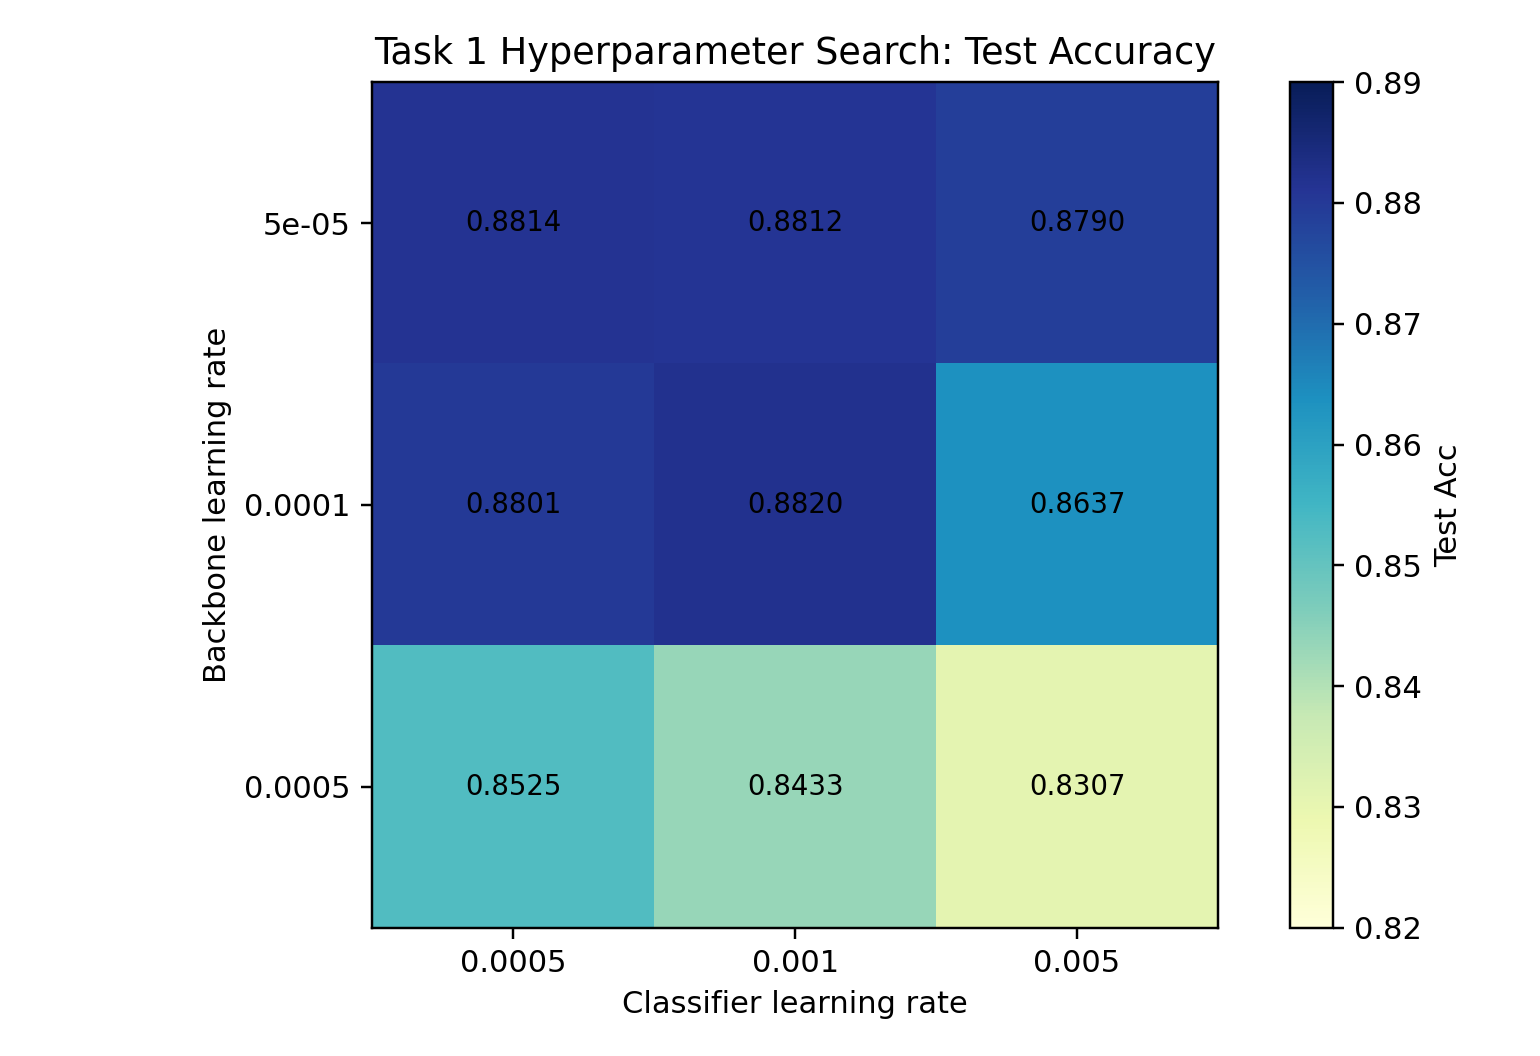
\includegraphics[width=0.78\textwidth]{assets/task1_hparam_heatmap.png}
\caption{任务 1 超参数搜索结果：不同学习率组合的测试准确率。}
\end{figure}

代表性结果如下表所示。主干学习率为 0.0001、分类层学习率为 0.001 时，测试准确率达到 0.8820，是本轮搜索中的最佳结果。主干学习率升至 0.0005 时准确率明显下降，说明微调预训练主干时更新幅度不宜过大，否则容易破坏 ImageNet 学到的通用特征。

\begin{table}[H]
\centering
\caption{任务 1 超参数搜索代表性结果}
\begin{tabular}{lrrrr}
\toprule
实验 & Epochs & Backbone LR & Classifier LR & Test Acc \\
\midrule
blr0.0001-clr0.001 & 15 & 0.0001 & 0.0010 & 0.8820 \\
blr0.00005-clr0.0005 & 15 & 0.00005 & 0.0005 & 0.8814 \\
blr0.00005-clr0.001 & 15 & 0.00005 & 0.0010 & 0.8812 \\
blr0.0001-clr0.0005 & 15 & 0.0001 & 0.0005 & 0.8801 \\
blr0.0005-clr0.001 & 15 & 0.0005 & 0.0010 & 0.8433 \\
\bottomrule
\end{tabular}
\end{table}

\subsection{训练曲线与验证 Accuracy}

\begin{figure}[H]
\centering
\begin{subfigure}{0.48\textwidth}
  \centering
  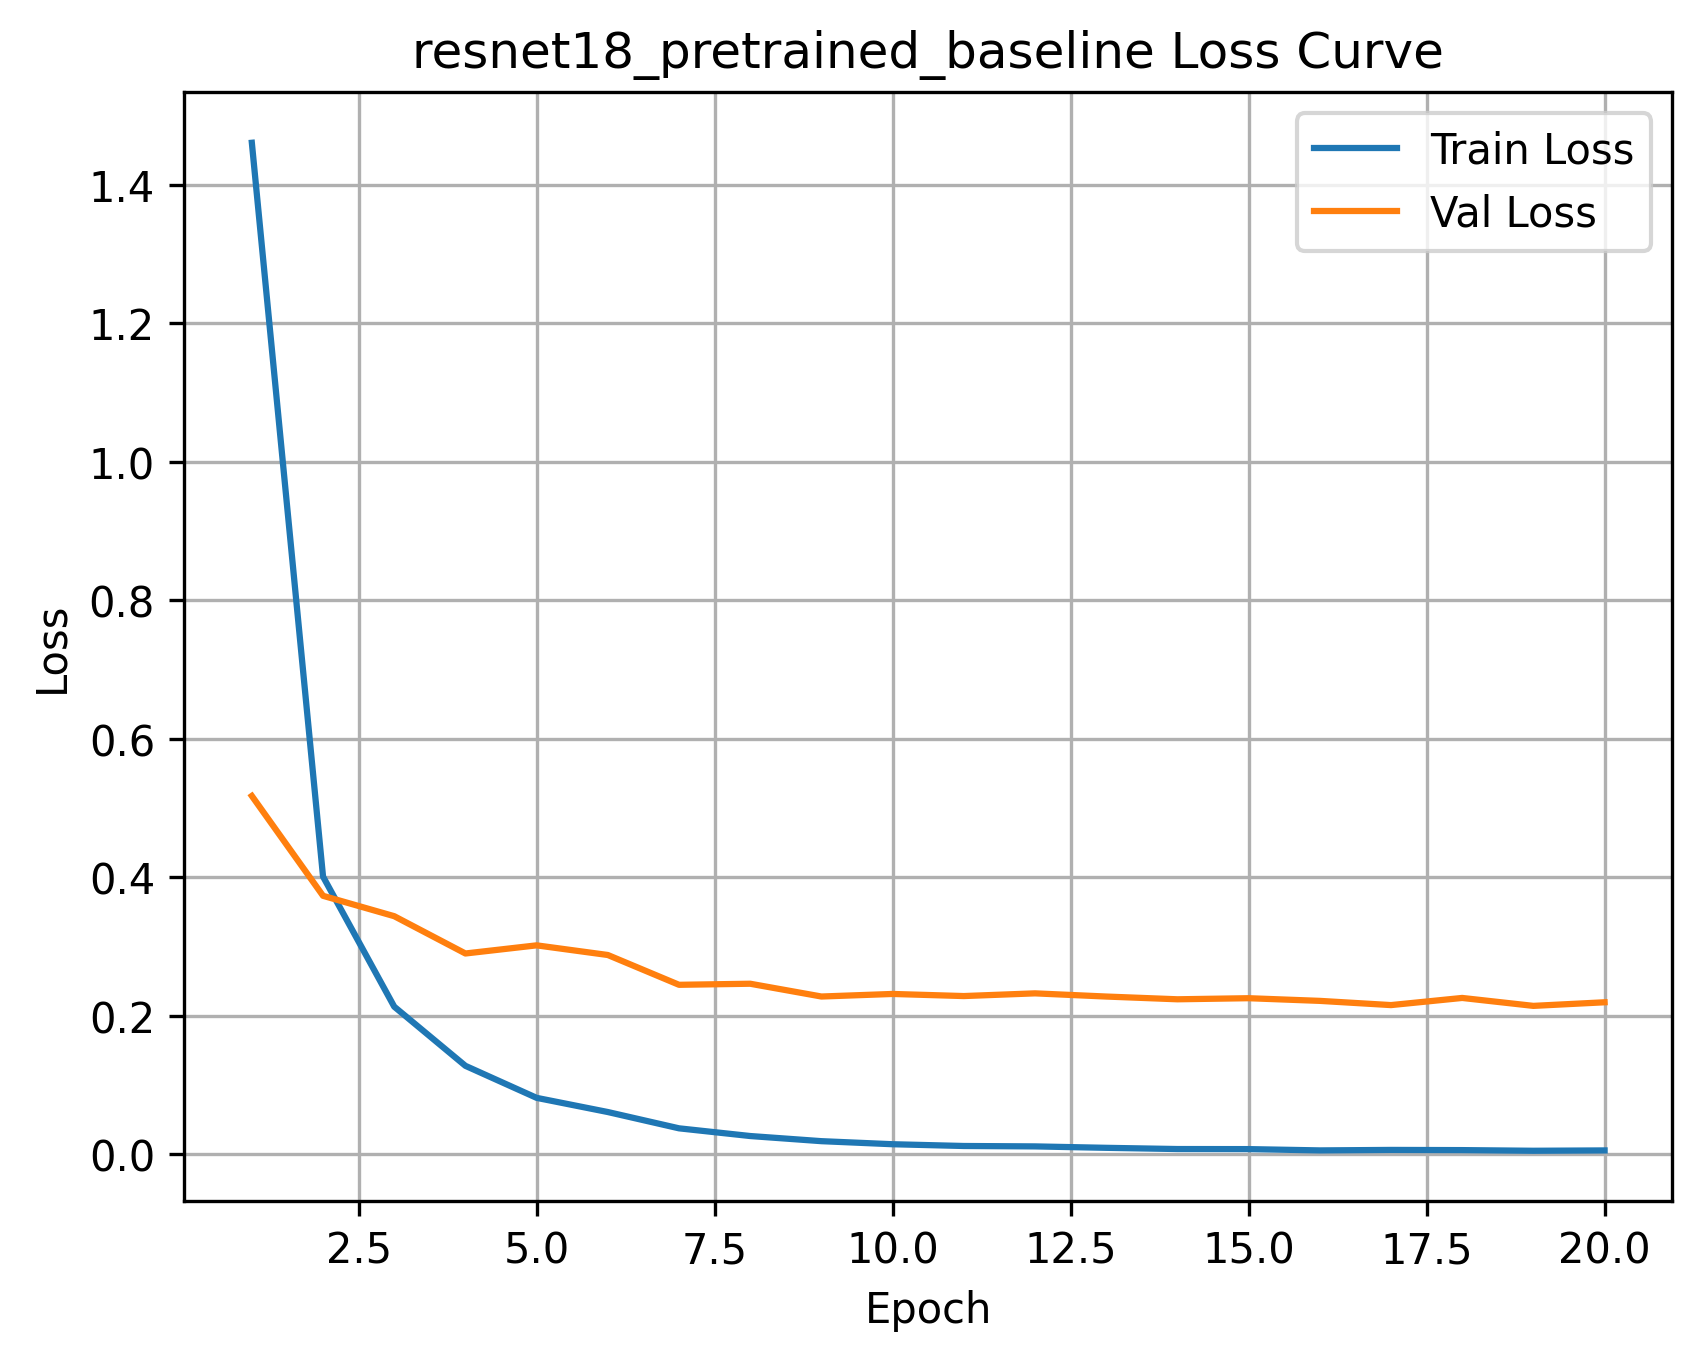
\includegraphics[width=\textwidth]{assets/task1_baseline_loss_curve.png}
  \caption{ResNet-18 loss 曲线}
\end{subfigure}
\hfill
\begin{subfigure}{0.48\textwidth}
  \centering
  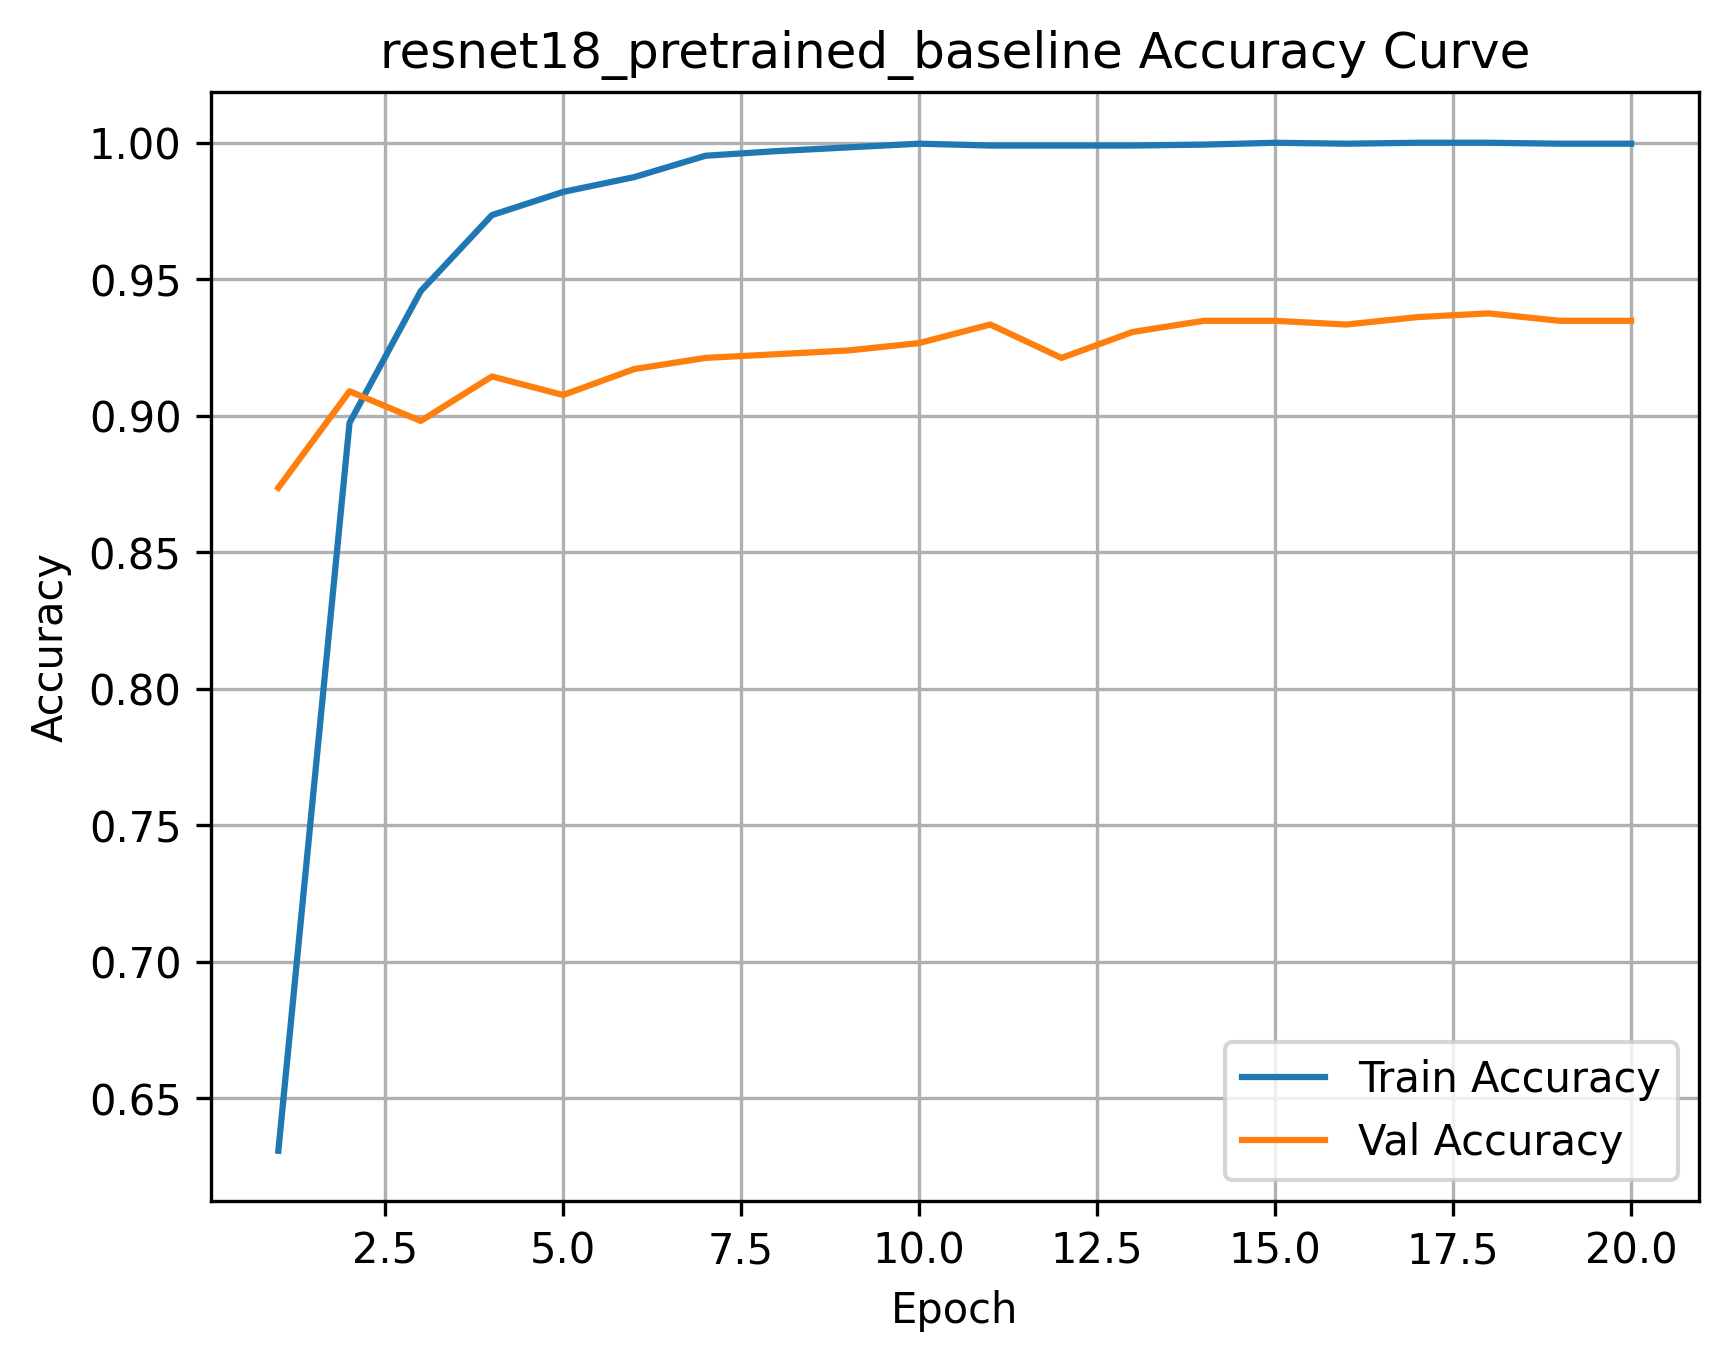
\includegraphics[width=\textwidth]{assets/task1_baseline_accuracy_curve.png}
  \caption{ResNet-18 accuracy 曲线}
\end{subfigure}
\caption{任务 1 Baseline 训练与验证可视化。}
\end{figure}

曲线显示，预训练 ResNet-18 的训练 loss 快速下降，训练准确率接近饱和，验证准确率稳定维持在较高水平。验证曲线与测试结果一致，说明 ImageNet 预训练特征对该细粒度分类任务有效。

\subsection{预训练消融与注意力机制}

预训练消融实验使用完全相同的 ResNet-18 结构与训练设置，对比 ImageNet 预训练初始化和随机初始化。注意力机制实验在 ResNet-18 的 BasicBlock 中加入手写 SE-block，将 SE-block 放在第二个 BatchNorm 之后、残差连接相加之前：

\begin{lstlisting}
conv1 -> bn1 -> relu -> conv2 -> bn2 -> SE-block -> residual add -> relu
\end{lstlisting}

由于加入 SE-block 后模型结构与 torchvision 原始 ResNet-18 不完全相同，因此仅加载名称和形状匹配的预训练参数，新增 SE-block 与新分类头从随机初始化开始训练。

\begin{figure}[H]
\centering
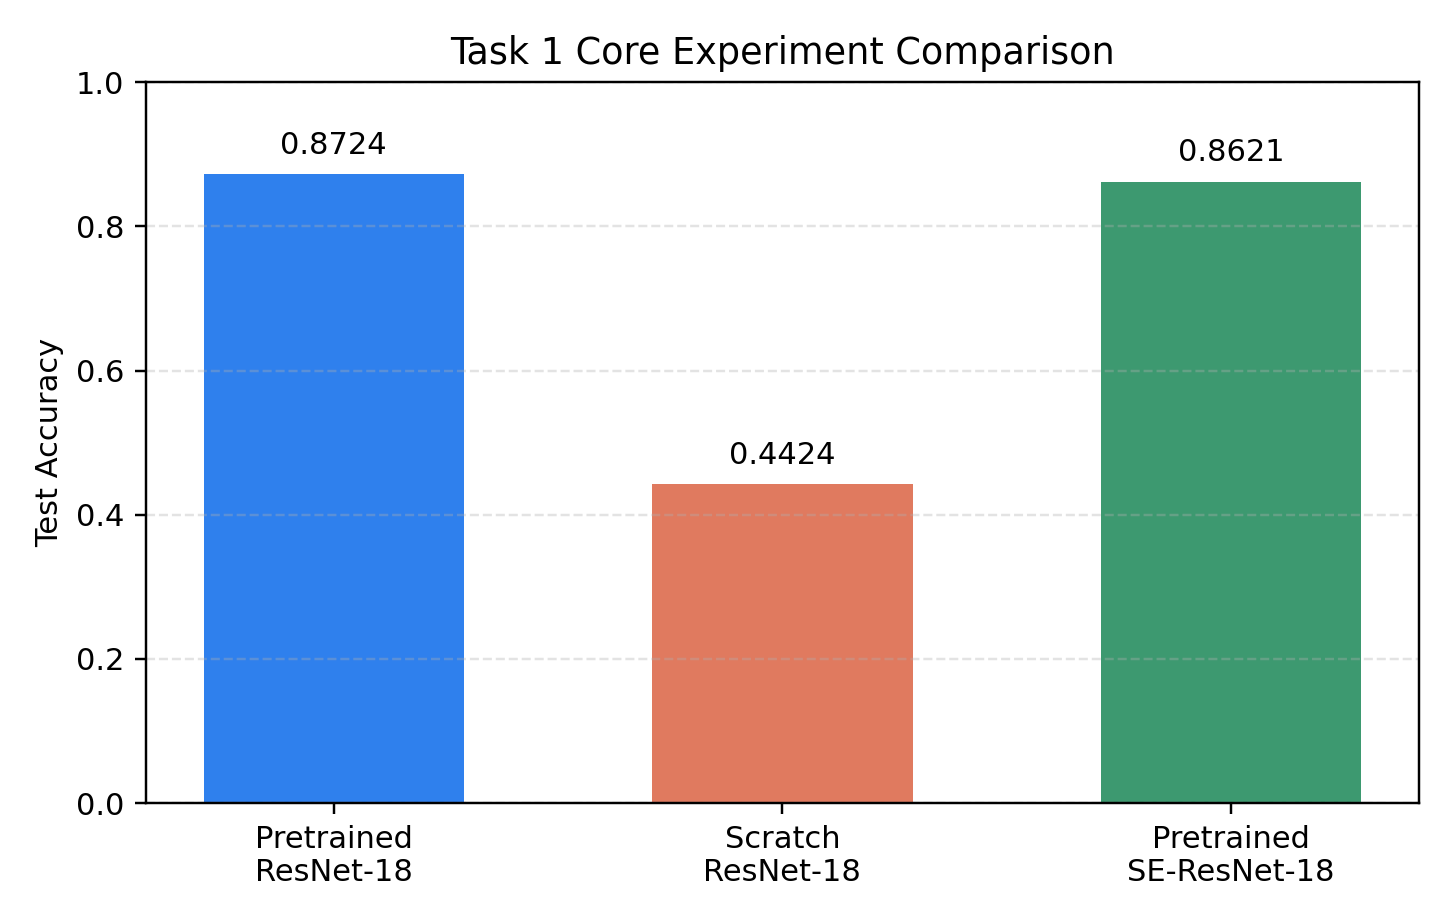
\includegraphics[width=0.72\textwidth]{assets/task1_core_comparison.png}
\caption{任务 1 核心实验测试准确率对比。}
\end{figure}

\begin{table}[H]
\centering
\caption{任务 1 核心实验结果}
\begin{tabular}{lccrr}
\toprule
实验 & 模型 & 预训练 & Best Val Acc & Test Acc \\
\midrule
Baseline & ResNet-18 & 是 & 0.9334 & 0.8724 \\
预训练消融 & ResNet-18 & 否 & 0.4959 & 0.4424 \\
注意力机制 & ResNet-18 + SE-block & 是 & 0.9063 & 0.8621 \\
\bottomrule
\end{tabular}
\end{table}

结果表明，ImageNet 预训练带来的收益最明显：与随机初始化相比，测试准确率提升约 43 个百分点。SE-block 版本测试准确率为 86.21\%，略低于原始 Baseline。这说明注意力机制在当前训练策略和数据规模下没有带来额外提升，可能原因包括新增参数带来过拟合风险、SE-block 无法直接继承原始 ResNet 权重，以及注意力模型未单独重新搜索学习率。

\section{任务 2：场景目标检测与视频多目标跟踪}

\subsection{任务目标与数据集}

任务 2 要求使用 VisDrone 无人机航拍检测数据集微调 YOLOv8 或同类单阶段检测模型，并将训练好的检测器用于 10--30 秒测试视频，实现逐帧检测、多目标跟踪、遮挡与 ID 跳变分析，以及基于 Tracking ID 的越线计数。

VisDrone 数据集中包含大量密集小目标，类别包括 pedestrian、people、bicycle、car、van、truck、tricycle、awning-tricycle、bus 和 motor。该数据集适合训练面向道路、行人和车辆场景的检测器。本实验使用 YOLOv8n 作为基础模型，主要考虑到其参数量较小、训练和推理开销低，适合在本地 RTX 4060 Ti 8GB 显存环境中完成实验流程。

\subsection{训练设置与工程实现}

训练前先进行了 1 epoch 测试训练以检查数据集路径、标签格式、GPU 调用和 YOLO 流程。由于 Windows 环境下多进程 DataLoader 在 Mosaic 数据增强中出现内存不足，正式训练采用较保守设置：\texttt{batch=4}、\texttt{workers=0}。正式模型命名为 \texttt{visdrone\_yolov8n\_e50}，训练 50 epoch。

\begin{table}[H]
\centering
\caption{任务 2 YOLOv8n 训练设置}
\begin{tabular}{ll}
\toprule
项目 & 设置 \\
\midrule
基础模型 & YOLOv8n \\
数据集 & VisDrone \\
Epochs & 50 \\
Input size & 640 \\
Batch size & 4 \\
Workers & 0 \\
Device & CUDA GPU \\
Optimizer & Ultralytics auto \\
主要指标 & Precision, Recall, mAP50, mAP50-95 \\
\bottomrule
\end{tabular}
\end{table}

\subsection{训练曲线与验证 mAP}

\begin{figure}[H]
\centering
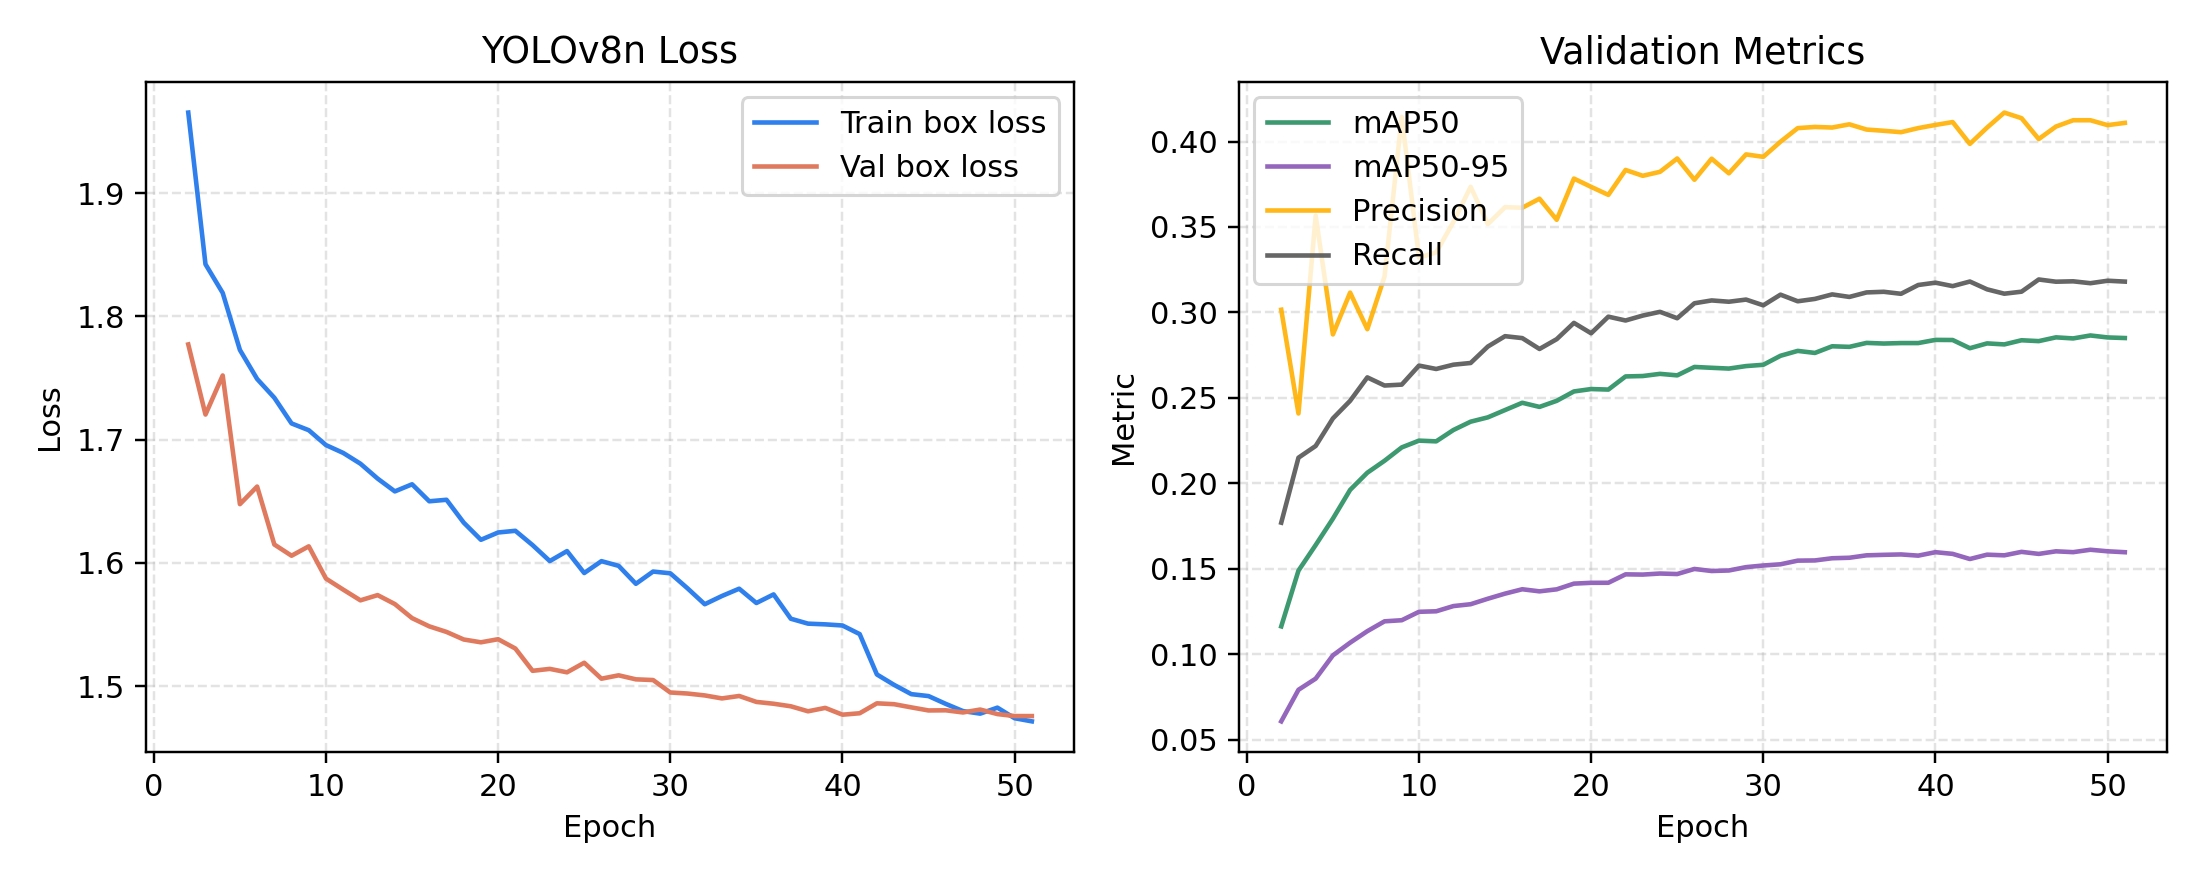
\includegraphics[width=0.95\textwidth]{assets/task2_training_curves.png}
\caption{任务 2 YOLOv8n 训练 loss 与验证指标曲线。}
\end{figure}

从训练曲线看，训练和验证 box loss 均持续下降；mAP50、mAP50-95、Precision 和 Recall 在前期提升较快，后期趋于平稳。最终整体 mAP50 约为 0.287，mAP50-95 约为 0.162，说明模型已经学习到基本检测能力，但 VisDrone 密集小目标任务仍较困难。

\begin{figure}[H]
\centering
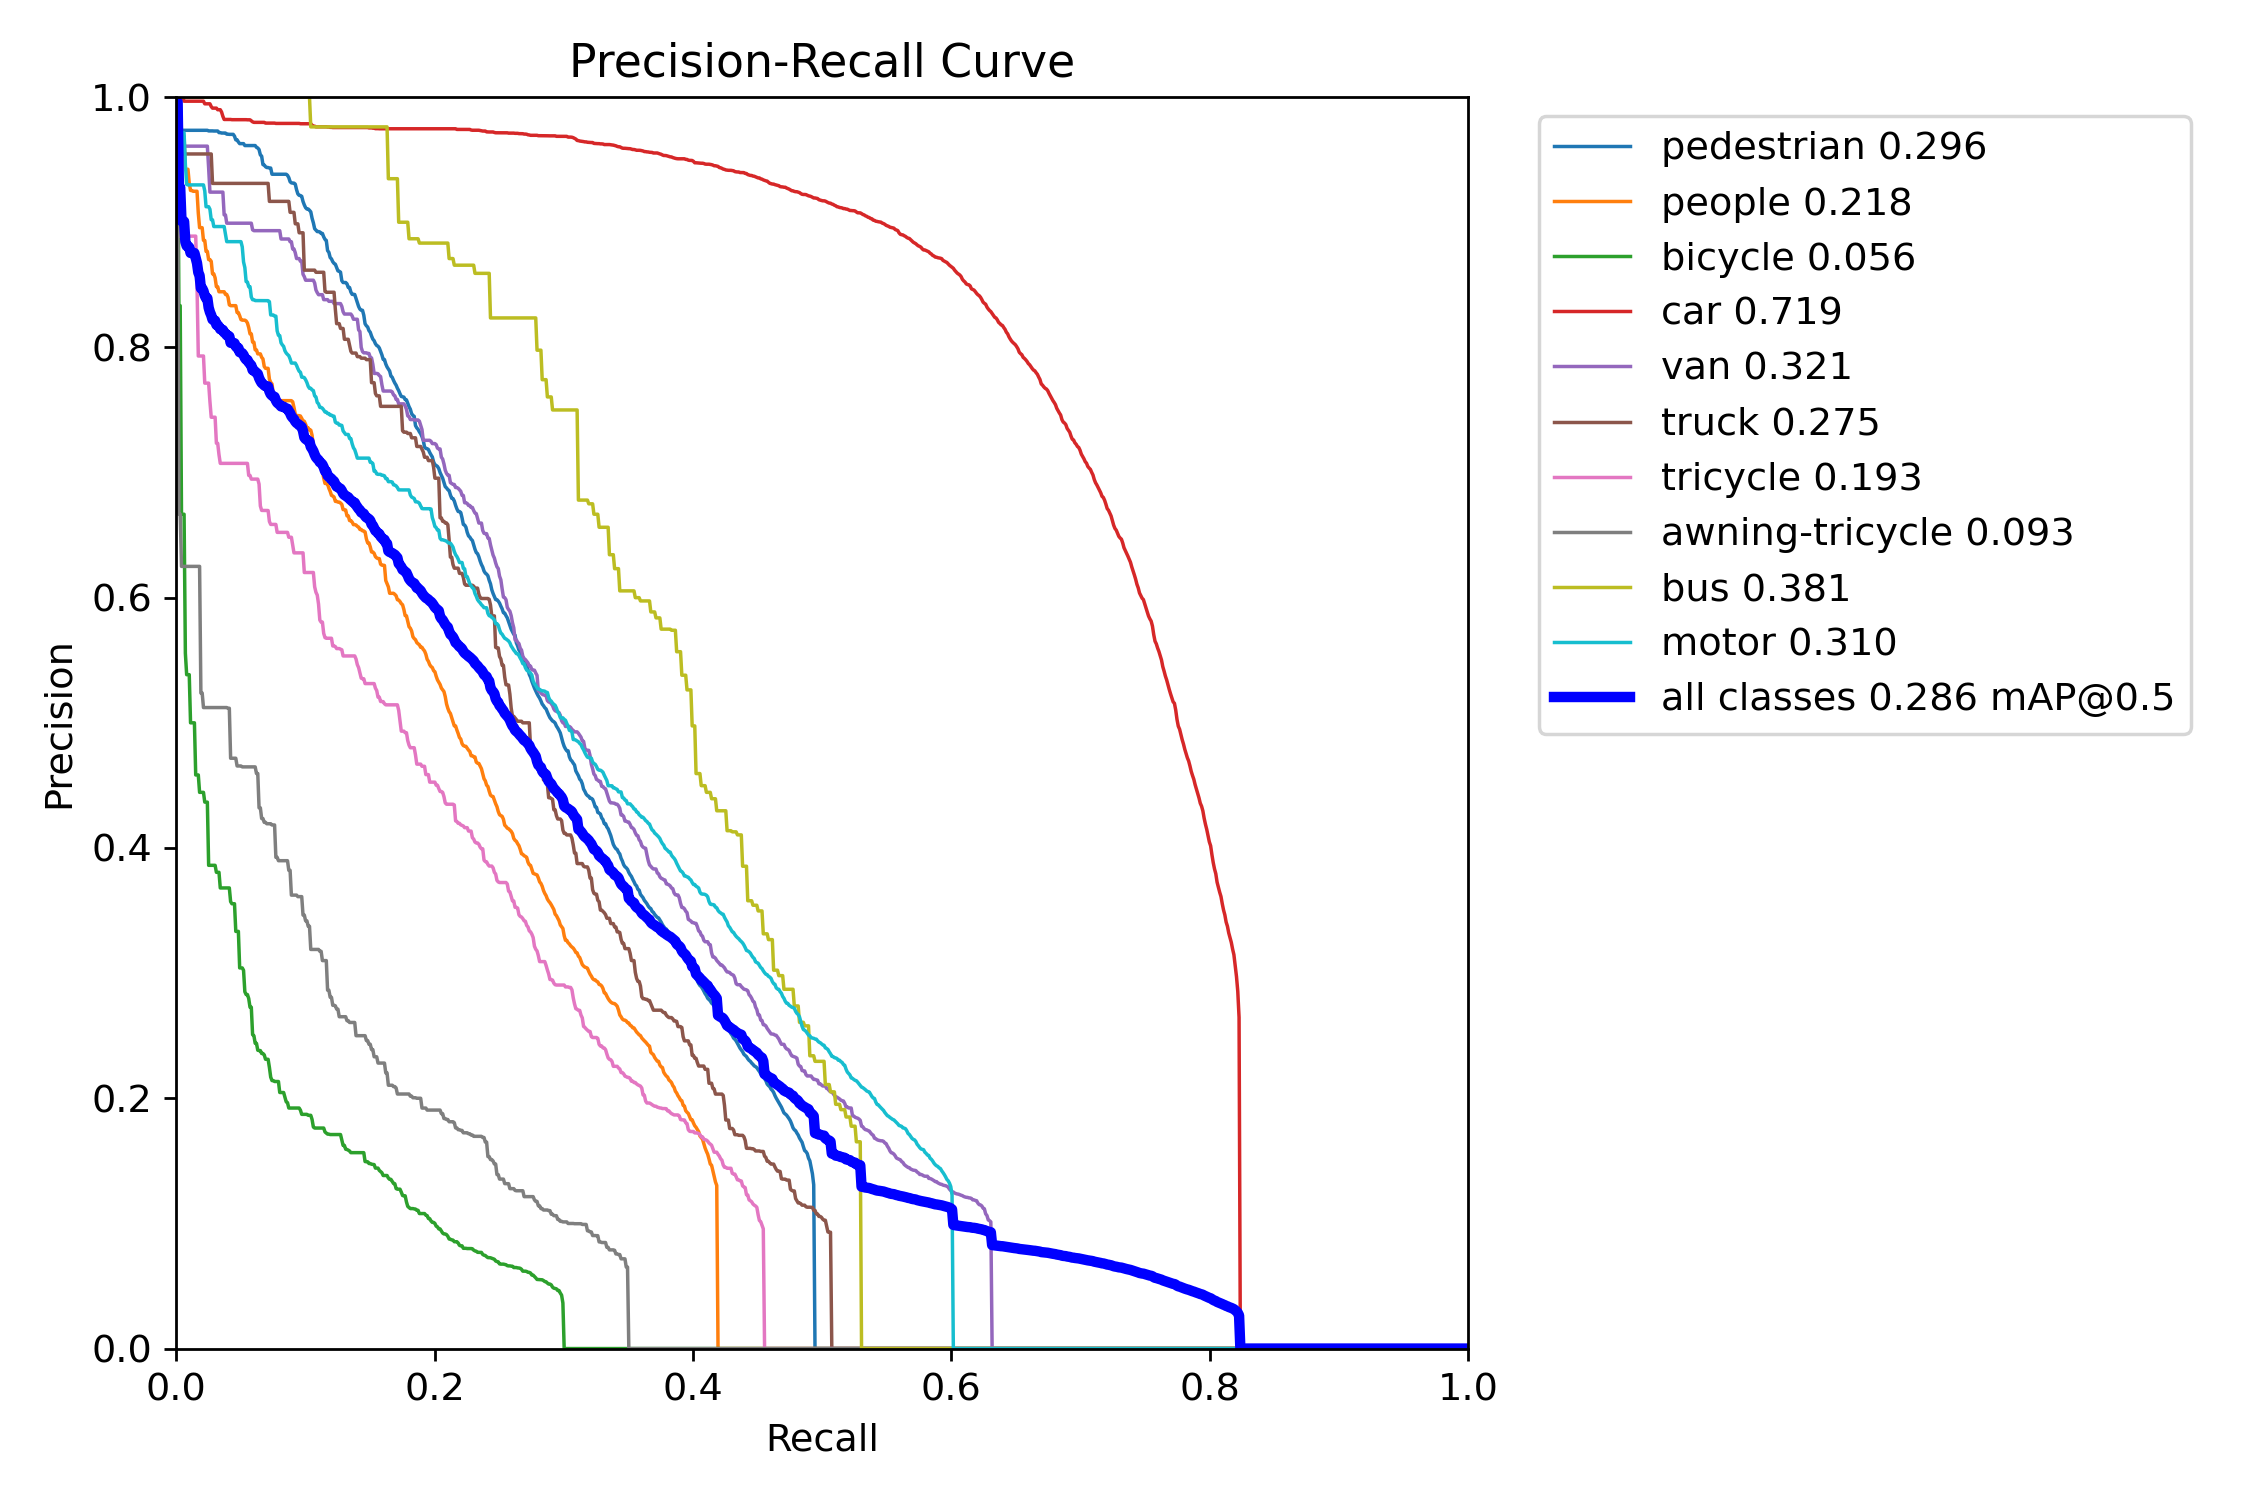
\includegraphics[width=0.72\textwidth]{assets/task2_box_pr_curve.png}
\caption{任务 2 验证集 PR 曲线。}
\end{figure}

\subsection{检测结果}

在 VisDrone 验证集上的主要结果如下：

\begin{table}[H]
\centering
\caption{任务 2 VisDrone 验证集检测结果}
\begin{tabular}{lrrrr}
\toprule
Class & Precision & Recall & mAP50 & mAP50-95 \\
\midrule
all & 0.412 & 0.318 & 0.287 & 0.162 \\
pedestrian & 0.398 & 0.342 & 0.297 & 0.119 \\
people & 0.476 & 0.233 & 0.222 & 0.073 \\
bicycle & 0.204 & 0.079 & 0.057 & 0.020 \\
car & 0.576 & 0.757 & 0.719 & 0.468 \\
van & 0.444 & 0.334 & 0.321 & 0.218 \\
truck & 0.440 & 0.292 & 0.276 & 0.180 \\
tricycle & 0.415 & 0.225 & 0.194 & 0.100 \\
awning-tricycle & 0.238 & 0.150 & 0.094 & 0.057 \\
bus & 0.515 & 0.398 & 0.382 & 0.260 \\
motor & 0.414 & 0.370 & 0.310 & 0.119 \\
\bottomrule
\end{tabular}
\end{table}

模型对 car 类别表现最好，mAP50 达到 0.719，Recall 达到 0.757；bicycle 和 awning-tricycle 表现较差，说明小型非机动车在密集航拍视角中更难检测和区分。这也解释了自采校园视频中电动车或自行车被误识别为 truck 的现象。

\begin{figure}[H]
\centering
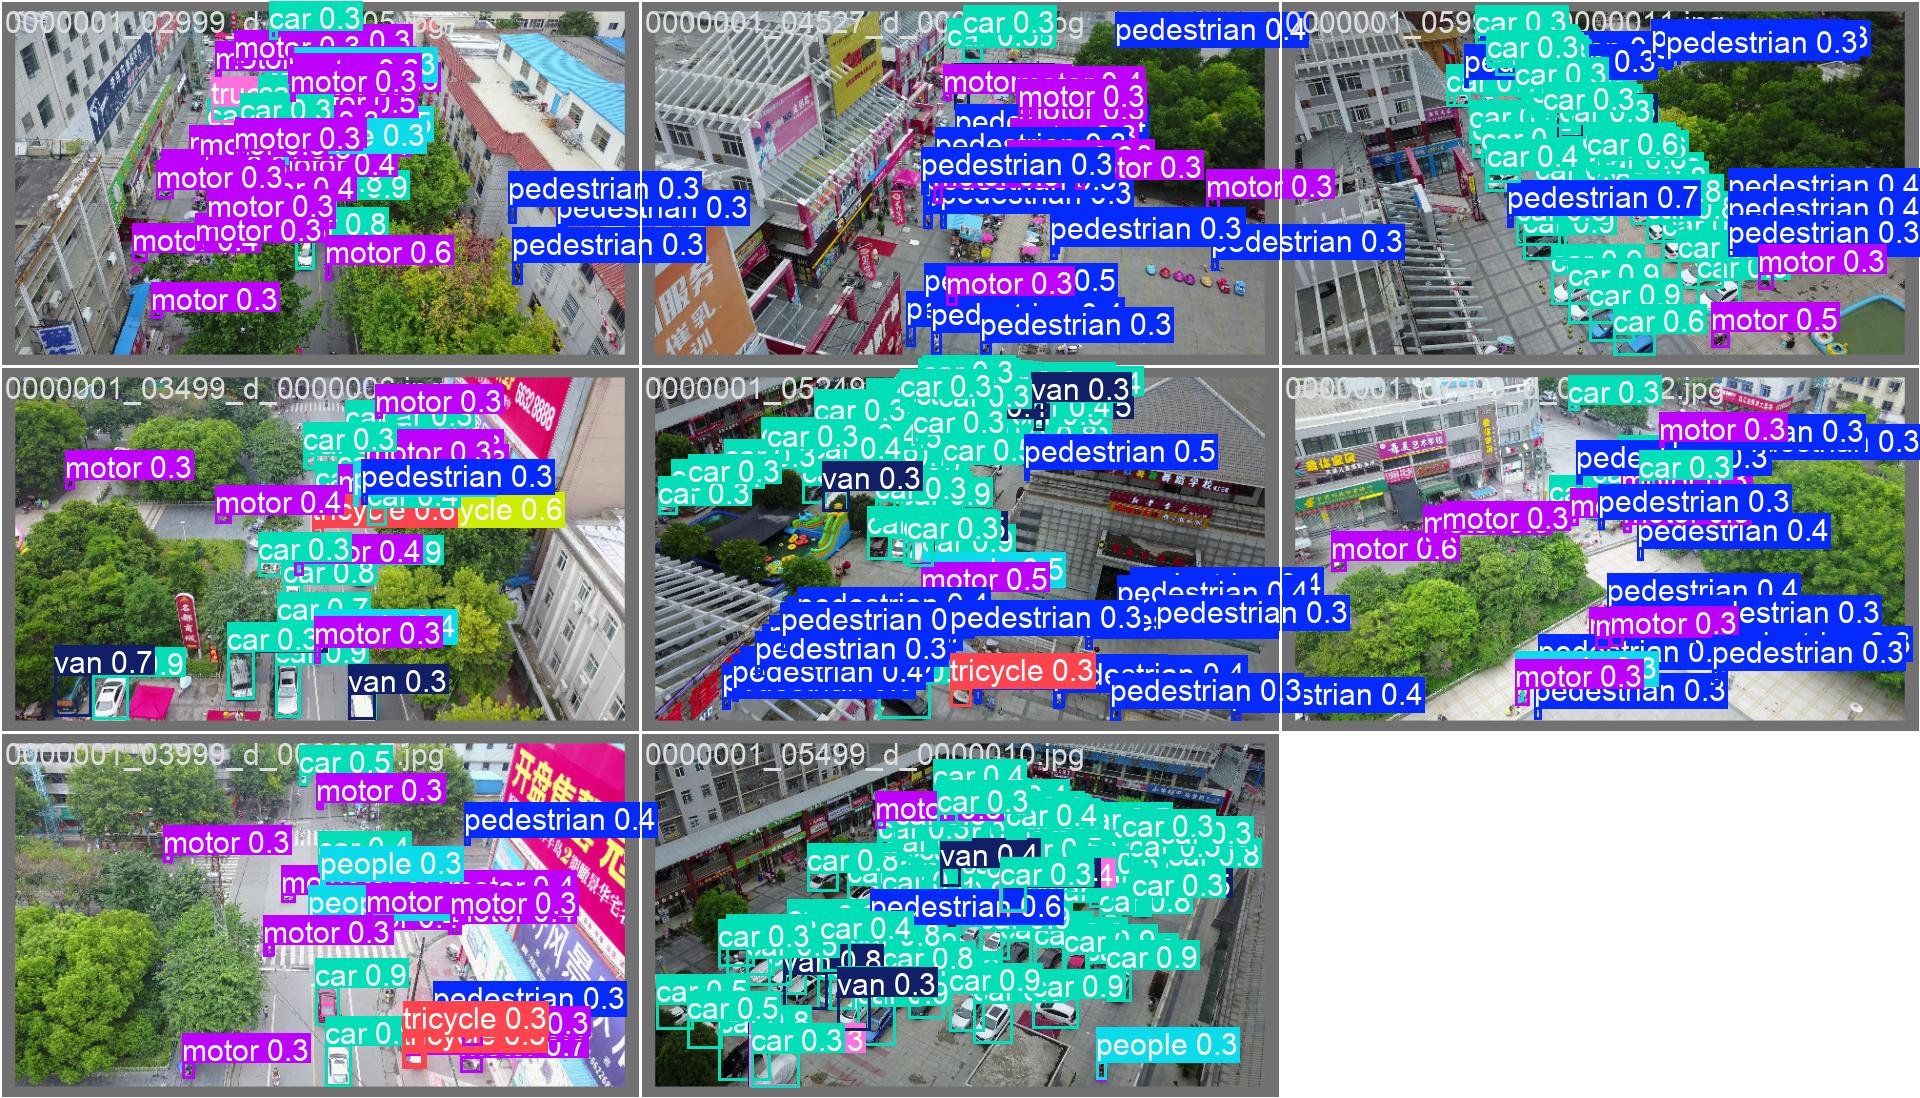
\includegraphics[width=0.9\textwidth]{assets/task2_val_prediction.jpg}
\caption{任务 2 验证集检测可视化示例。}
\end{figure}

\subsection{视频多目标跟踪}

完成检测模型训练后，实验使用自采校园道路视频作为测试视频。该视频包含行人、电动车、道路、树木、建筑物、灌木和阴影。测试场景与 VisDrone 存在明显域差异：VisDrone 主要是无人机俯视航拍，而测试视频更接近地面或路边视角；同时树叶、阴影和背景纹理对检测造成干扰。

视频推理使用 YOLOv8 内置 tracking，设置 \texttt{persist=True} 保持帧间轨迹连续。输出视频中每个目标包含 bounding box、类别、置信度和 Tracking ID。部分行人在连续帧中能保持稳定 ID，满足多目标跟踪基本要求；但也存在背景误检、类别混淆、检测框抖动和短时漏检。

\subsection{遮挡与 ID 跳变分析}

根据任务要求，实验从跟踪视频中截取了连续遮挡片段。如下图所示，电动车目标在 Frame 586 被检测并分配 ID 29；随后几帧中检测框短暂消失，说明遮挡、背景干扰或置信度下降导致目标丢失。

\begin{figure}[H]
\centering
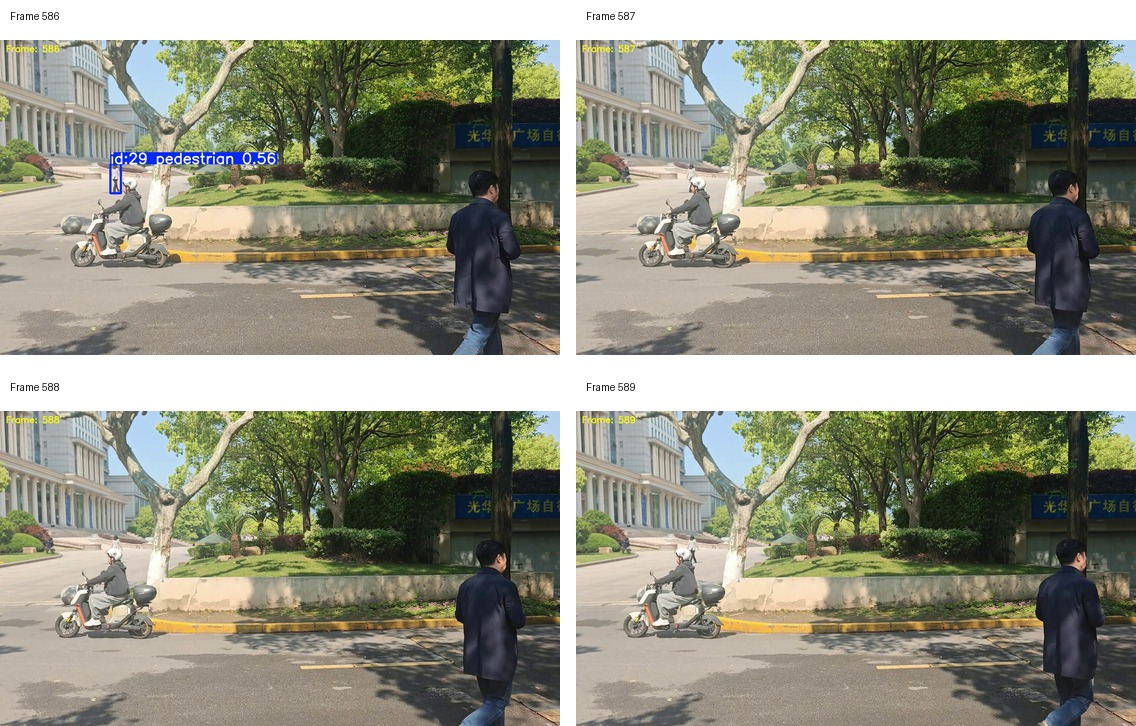
\includegraphics[width=0.95\textwidth]{assets/task2_occlusion_montage.jpg}
\caption{任务 2 遮挡片段连续帧可视化。}
\end{figure}

该片段中没有观察到明显的 ID switch：目标重新出现时未被错误分配给另一个已有目标，也没有出现两个目标交换 ID 的情况。主要问题是检测器对遮挡目标召回不足，导致目标框短时中断。多目标跟踪依赖检测结果、运动预测和帧间匹配；当检测框消失时，跟踪器只能依赖短期轨迹缓存维持目标，遮挡较短时可能恢复原有 ID，遮挡较长或相似目标交汇时则更容易发生 ID switch。

\subsection{越线计数}

越线计数在视频画面中设置一条竖直虚拟线，记录每个 Tracking ID 上一帧和当前帧中心点位于线的哪一侧。如果同一 ID 从线的一侧移动到另一侧，且该 ID 尚未被计数，则总计数加一。程序维护已计数 ID 集合，避免同一目标重复计数。

\begin{figure}[H]
\centering
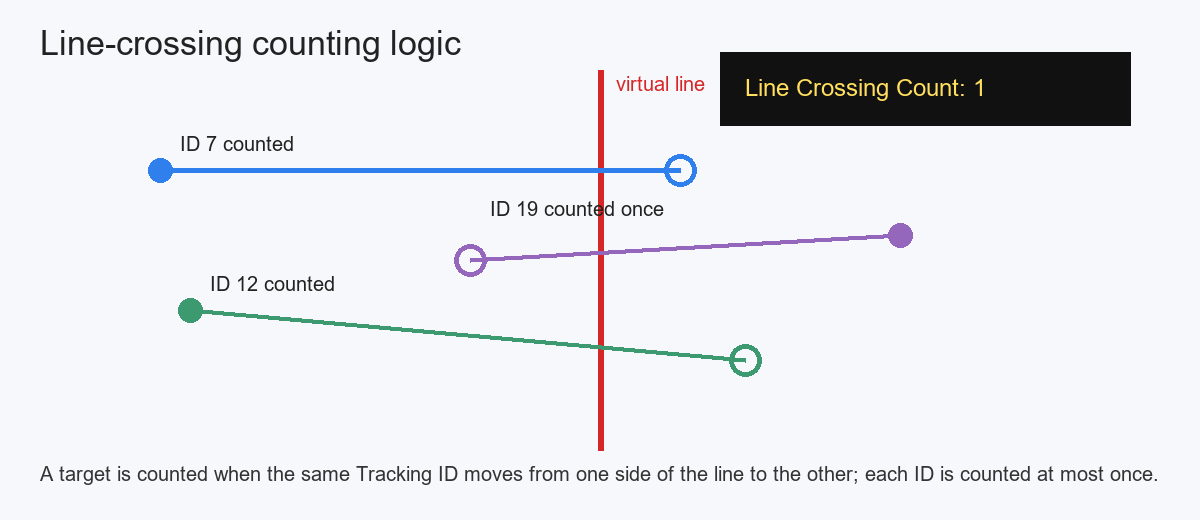
\includegraphics[width=0.85\textwidth]{assets/task2_line_count_logic.png}
\caption{任务 2 越线计数逻辑示意图。}
\end{figure}

实际测试视频中，人工观察约有 3 个目标穿过虚拟线，而程序统计结果为 1。偏差主要来自检测和跟踪不稳定：目标靠近虚拟线时若发生漏检、类别突变或 ID 轨迹中断，程序无法获得完整的线前和线后位置，越线逻辑就不会触发。后续可通过提高检测模型性能、调整置信度阈值、优化 tracker 参数、增加轨迹缓存和多帧平滑来提升计数准确性。

\section{任务 3：从零搭建 U-Net 与损失函数工程}

\subsection{任务目标与数据集}

任务 3 要求不使用任何预训练权重，使用深度学习框架基础 API 从零手写 U-Net，包括下采样编码器、上采样解码器和 Skip Connection；在 Oxford-IIIT Pet Dataset 三分类分割任务上训练，并手动实现 Dice Loss，比较 CE、Dice、CE + Dice 三种损失配置在验证集上的 mIoU。

本实验使用 Oxford-IIIT Pet 的 segmentation trimap 标注。原始 mask 像素值通常为 1、2、3，分别对应宠物主体、背景和边界。实验将其减 1 映射为 0、1、2 三类，以适配 \texttt{nn.CrossEntropyLoss()}。输入图像与 mask 统一 resize 为 $256\times256$；图像 resize 使用双线性插值，mask resize 使用最近邻插值，避免产生非整数类别标签。

\subsection{U-Net 网络结构}

U-Net 由编码器、解码器和输出层组成。基本模块为 DoubleConv，即连续两次 \texttt{Conv2d -> BatchNorm2d -> ReLU}。下采样模块由 \texttt{MaxPool2d} 与 DoubleConv 组成；上采样模块使用 \texttt{ConvTranspose2d} 放大特征图，与对应编码器层在 channel 维度拼接，再通过 DoubleConv 融合。最终使用 $1\times1$ 卷积输出三分类 logits。

\begin{lstlisting}[language=Python]
x1 = self.in_conv(x)
x2 = self.down1(x1)
x3 = self.down2(x2)
x4 = self.down3(x3)
x5 = self.down4(x4)

x = self.up1(x5, x4)
x = self.up2(x, x3)
x = self.up3(x, x2)
x = self.up4(x, x1)

logits = self.out_conv(x)
\end{lstlisting}

Skip Connection 的核心是：

\begin{lstlisting}[language=Python]
x = torch.cat([skip, x], dim=1)
\end{lstlisting}

深层特征提供语义信息，浅层特征保留边缘、轮廓和位置细节，因此 Skip Connection 对像素级分割尤为重要。模型测试中，输入形状 $[2,3,256,256]$ 时输出为 $[2,3,256,256]$，满足逐像素三分类要求。

\subsection{Dice Loss 手动实现}

Dice 系数衡量预测区域与真实区域的重叠程度：

\[
Dice = \frac{2|P\cap G|}{|P|+|G|}
\]

Dice Loss 定义为：

\[
DiceLoss = 1 - Dice
\]

多分类实现时，先对 logits 做 softmax 得到类别概率，再将标签转为 one-hot 形式并计算各类别 Dice，最后对类别取平均。核心实现如下：

\begin{lstlisting}[language=Python]
probs = torch.softmax(logits, dim=1)
targets_one_hot = F.one_hot(targets, num_classes=self.num_classes)
targets_one_hot = targets_one_hot.permute(0, 3, 1, 2).float()

intersection = torch.sum(probs * targets_one_hot, dim=(0, 2, 3))
cardinality = torch.sum(probs + targets_one_hot, dim=(0, 2, 3))
dice_score = (2.0 * intersection + smooth) / (cardinality + smooth)
dice_loss = 1.0 - dice_score.mean()
\end{lstlisting}

组合损失为 Cross-Entropy Loss + Dice Loss。CE 提供稳定的逐像素分类梯度，Dice Loss 强化区域重叠优化，两者互补，理论上更适合存在类别像素不均衡的分割任务。

\subsection{训练设置}

\begin{table}[H]
\centering
\caption{任务 3 U-Net 训练设置}
\begin{tabular}{ll}
\toprule
项目 & 设置 \\
\midrule
数据集 & Oxford-IIIT Pet segmentation trimap \\
任务 & 三分类语义分割 \\
输入尺寸 & $256\times256$ \\
模型 & 从零训练 U-Net \\
Base channels & 64 \\
Batch size & 8 \\
Epochs & 50 \\
Optimizer & AdamW \\
Learning rate & 0.0001 \\
Weight decay & 0.0001 \\
损失函数 & CE / Dice / CE + Dice \\
评价指标 & Pixel Accuracy, class IoU, mIoU \\
\bottomrule
\end{tabular}
\end{table}

\subsection{训练曲线与 mIoU 对比}

\begin{figure}[H]
\centering
\begin{subfigure}{0.48\textwidth}
  \centering
  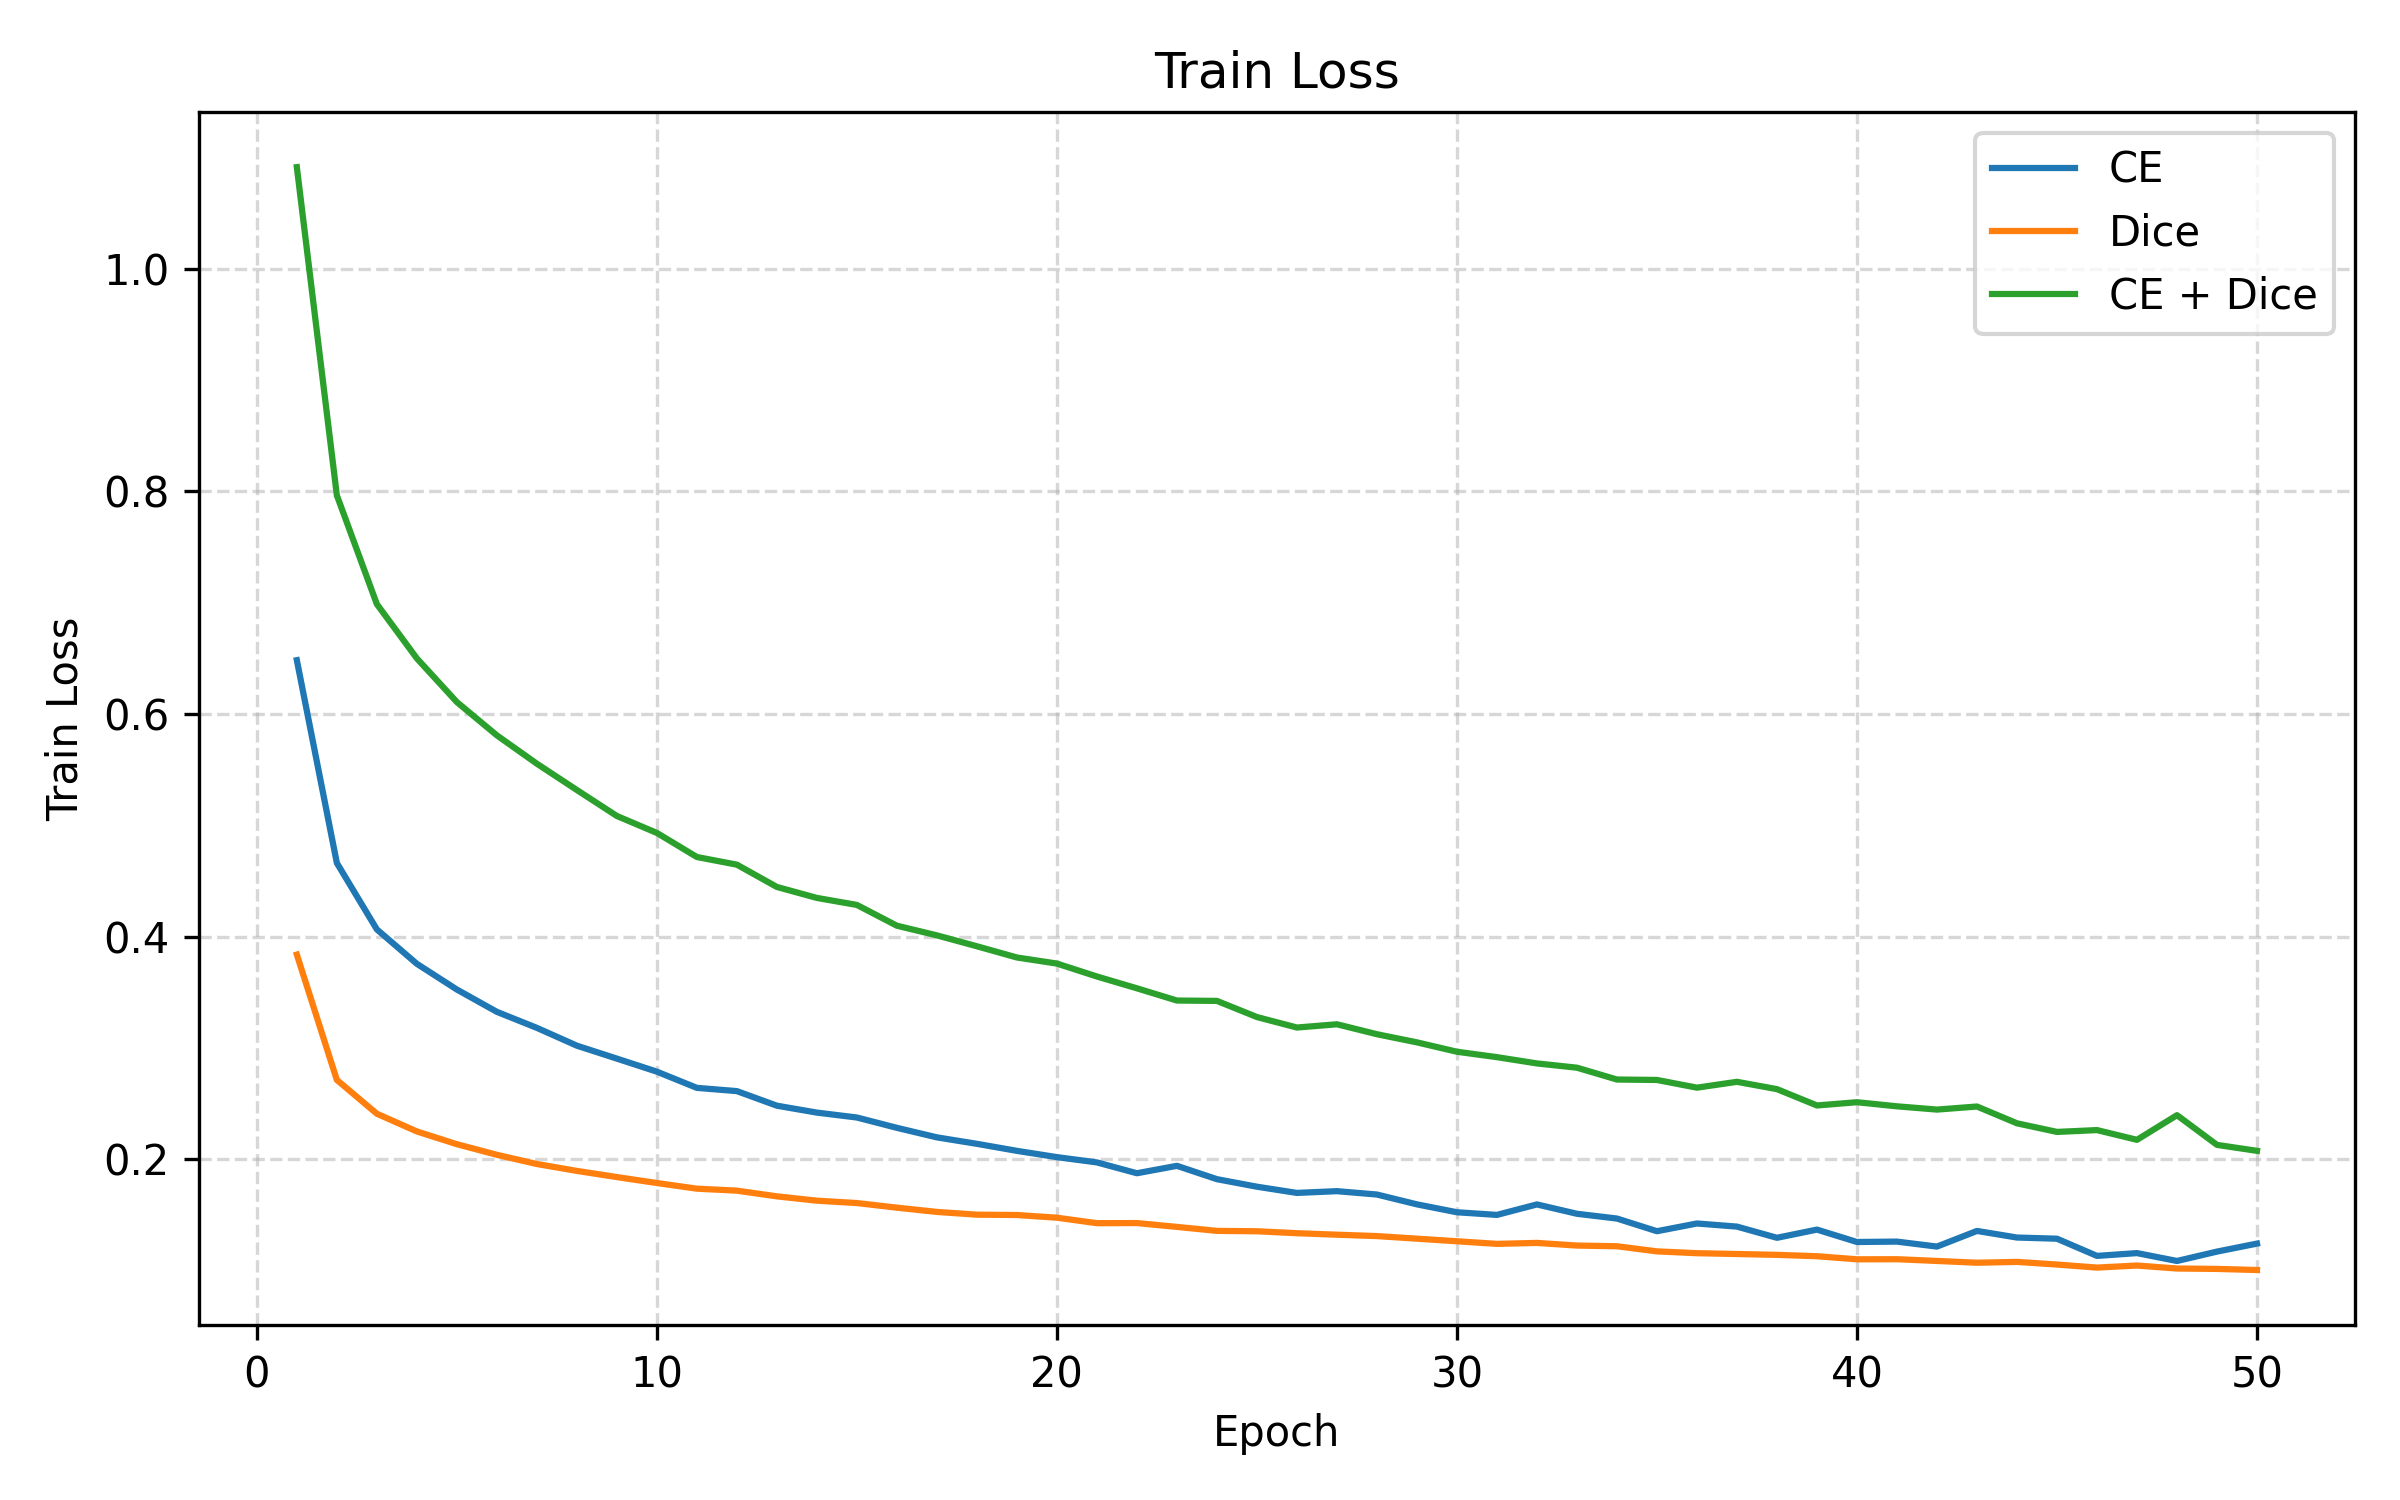
\includegraphics[width=\textwidth]{assets/task3_train_loss_comparison.png}
  \caption{Train loss}
\end{subfigure}
\hfill
\begin{subfigure}{0.48\textwidth}
  \centering
  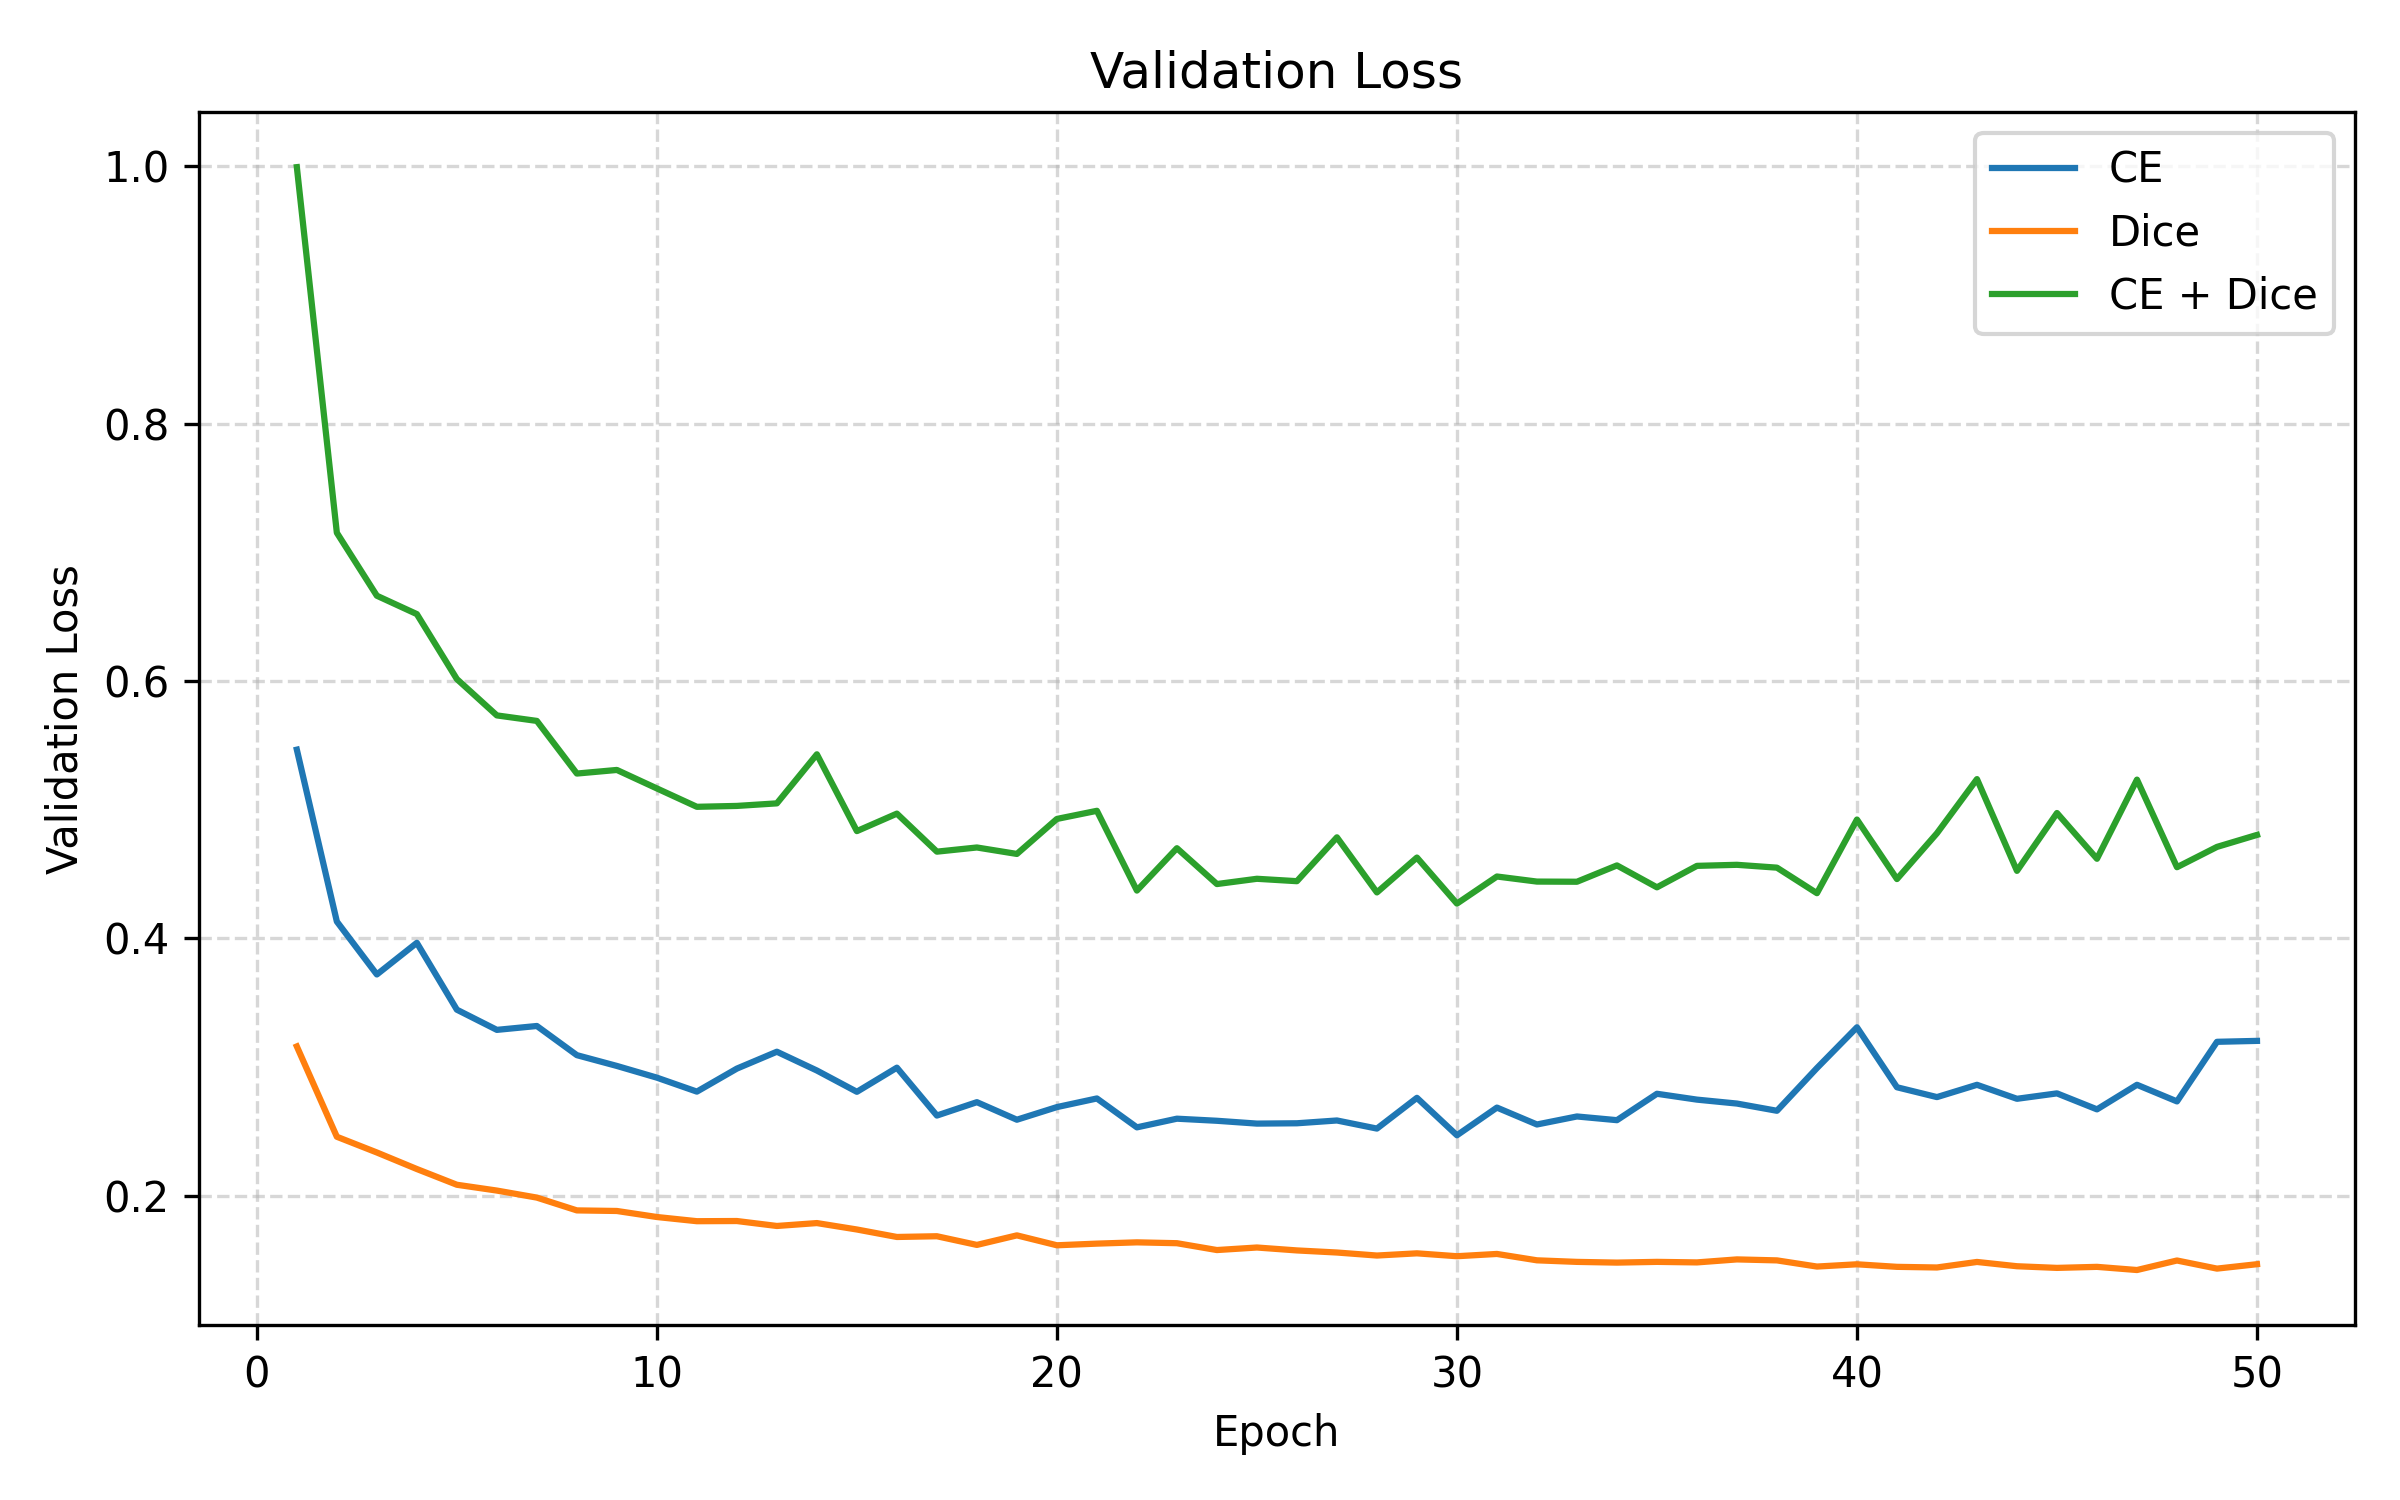
\includegraphics[width=\textwidth]{assets/task3_val_loss_comparison.png}
  \caption{Validation loss}
\end{subfigure}
\caption{任务 3 三种损失配置的 loss 曲线。}
\end{figure}

\begin{figure}[H]
\centering
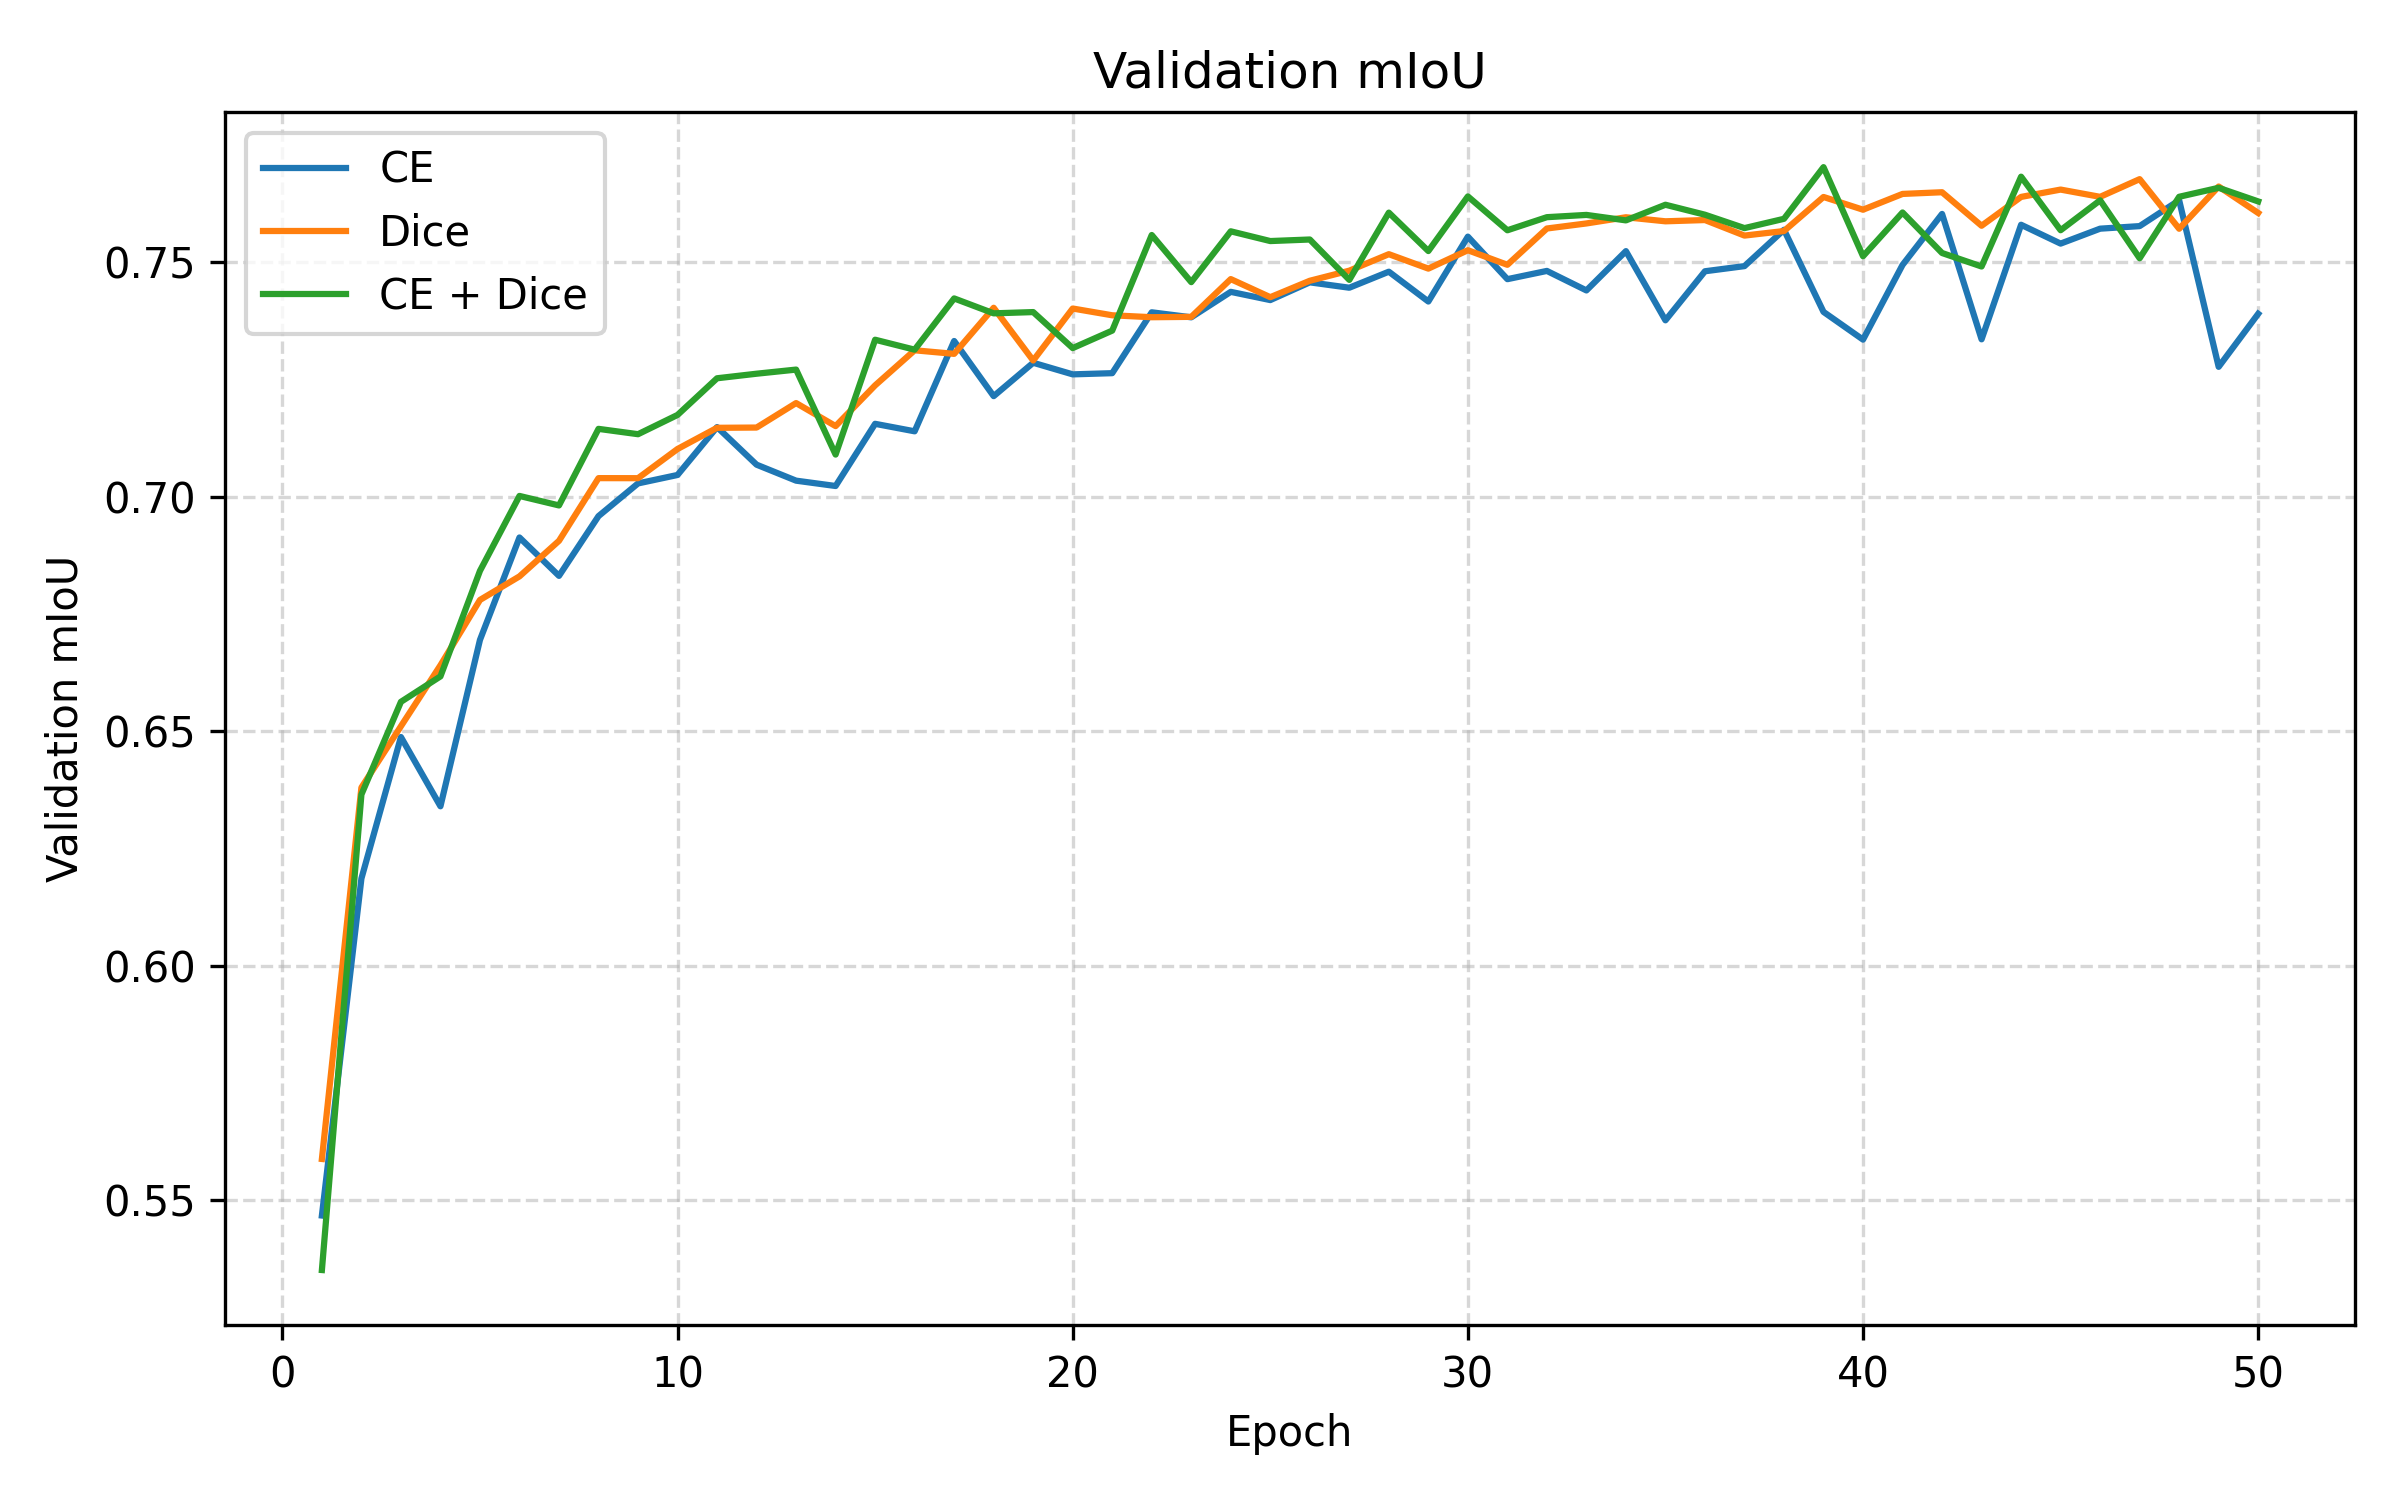
\includegraphics[width=0.72\textwidth]{assets/task3_val_miou_comparison.png}
\caption{任务 3 三种损失配置的验证集 mIoU 曲线。}
\end{figure}

\begin{table}[H]
\centering
\caption{任务 3 三种损失函数配置结果}
\begin{tabular}{lrrrr}
\toprule
Loss Config & Best Val mIoU & Best Epoch & Final Val mIoU & Final Pixel Acc \\
\midrule
CE & 0.763213 & 48 & 0.738991 & 0.900209 \\
Dice & 0.767711 & 47 & 0.760501 & 0.909191 \\
CE + Dice & 0.770272 & 39 & 0.762963 & 0.912962 \\
\bottomrule
\end{tabular}
\end{table}

结果显示，CE + Dice 取得最高 Best Val mIoU，为 0.770272；Dice Loss 单独使用时为 0.767711；CE 为 0.763213。三者差距不大，但趋势清晰：加入 Dice Loss 后 mIoU 提升，组合损失效果最好，并且在第 39 epoch 更早达到最佳验证表现。

\subsection{类别 IoU 与可视化分析}

以 CE + Dice 最后一轮为例，三类 IoU 为 0.840958、0.911047、0.536885。模型对大面积区域表现较好，尤其是背景和宠物主体；边界类 IoU 明显较低，因为 trimap 边界通常是一圈较窄像素带，面积小、形状复杂，且更容易受到 resize、标注精度和上采样误差影响。

\begin{figure}[H]
\centering
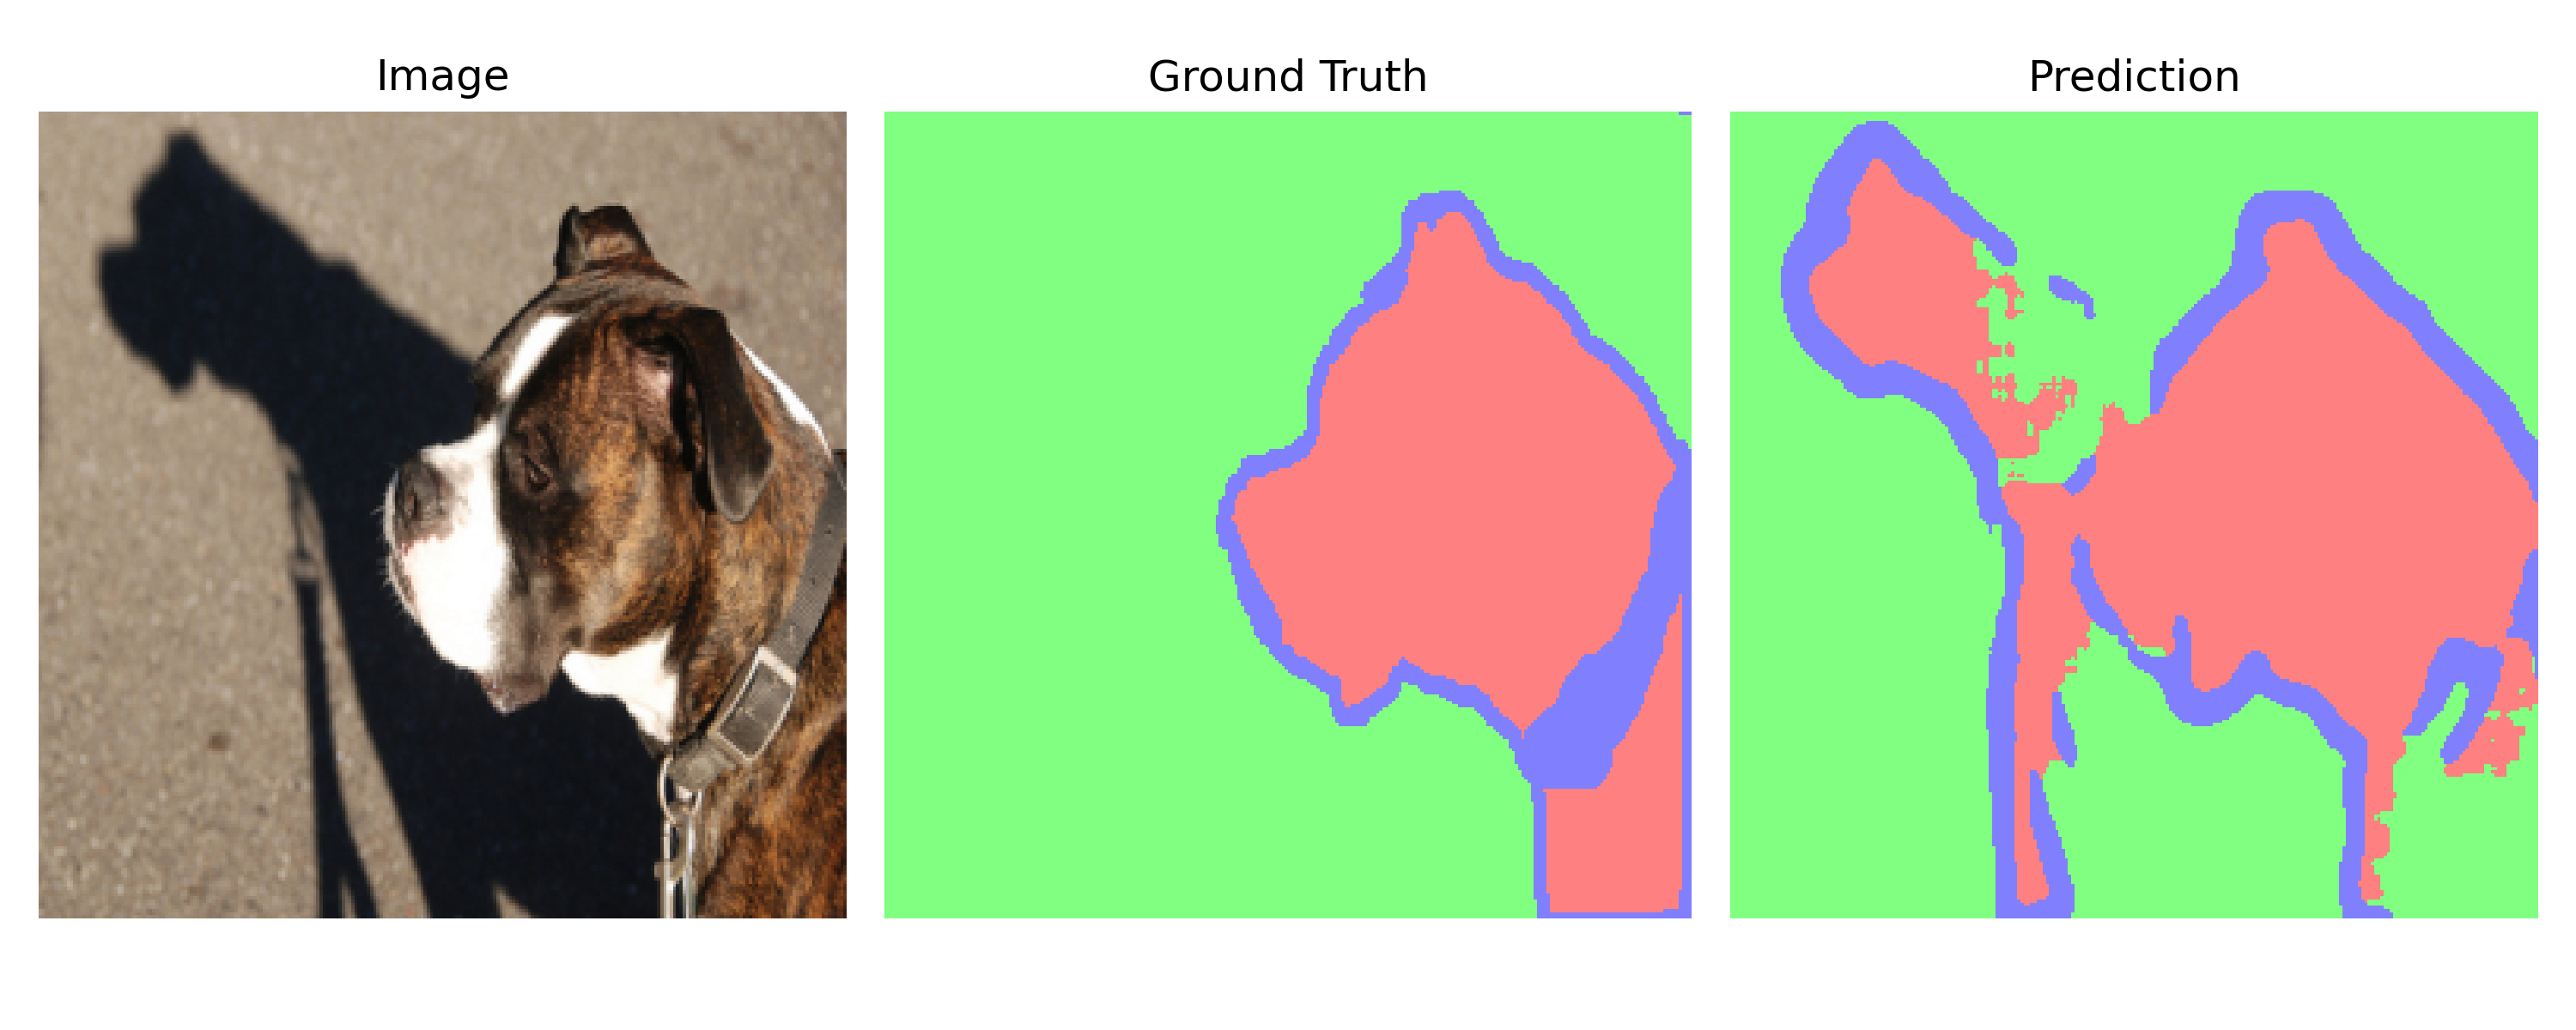
\includegraphics[width=0.86\textwidth]{assets/task3_prediction_example.png}
\caption{任务 3 CE + Dice 模型在验证集上的预测可视化：原图、真实 mask 与预测 mask。}
\end{figure}

可视化结果与数值指标一致：模型能较稳定地分割宠物主体与背景，但在边界、腿部、阴影和细长结构附近容易出现局部误分割。由于实验要求从随机初始化开始训练，当前结果说明手写 U-Net 已经能够在轻量级分割数据集上有效收敛。

\section{总结}

任务 1 中，预训练 ResNet-18 在 Oxford-IIIT Pet 细粒度分类上显著优于随机初始化模型，说明迁移学习对中小规模视觉任务非常关键。超参数搜索表明 backbone learning rate 不宜过大，0.0001 与分类头学习率 0.001 是较稳健的组合。SE-block 完成了注意力机制引入要求，但在当前设置下未超过 Baseline。

任务 2 中，YOLOv8n 在 VisDrone 上完成 50 epoch 微调，获得整体 Precision 0.412、Recall 0.318、mAP50 0.287、mAP50-95 0.162。自采视频中能够输出检测框、类别与 Tracking ID，并实现遮挡分析和越线计数，但受域差异、误检、漏检和 ID 连续性影响，实际计数结果低于人工观察值。

任务 3 中，手写 U-Net 完成了无预训练语义分割训练，并手动实现 Dice Loss。CE + Dice 组合损失取得最高验证 mIoU 0.770272，验证了 Dice Loss 在类别不均衡分割任务中的价值，也说明组合损失能兼顾像素分类准确性和区域重叠质量。

整体来看，本次作业完整覆盖了分类、检测跟踪和分割三类计算机视觉任务，代码、训练结果、可视化图、模型权重与复现说明均已整理到仓库与网盘中。

\end{document}
